\documentclass[11pt,british]{report}
\renewcommand{\rmdefault}{ptm}
\renewcommand{\familydefault}{\rmdefault}
%formatting packages
\usepackage[T1]{fontenc}
\usepackage[latin9]{inputenc}
\usepackage[a4paper]{geometry}
\geometry{verbose,tmargin=3cm,bmargin=3cm,lmargin=3.5cm,rmargin=2.4cm}
\usepackage{fancyhdr}
\pagestyle{fancy}
\setcounter{secnumdepth}{3}
\usepackage[british]{babel}
\usepackage{booktabs}
\usepackage{array,multirow}
\usepackage{subfig}
\usepackage[explicit]{titlesec}
\usepackage{adjustbox}
\usepackage{cite}
\usepackage{pdfpages}
\usepackage{standalone}
\usepackage[toc,page]{appendix}
\usepackage{listings}
\usepackage{setspace}
\usepackage{acro}
\usepackage{etoolbox}

%%maths
\usepackage{units}
\usepackage{siunitx}
\usepackage{amsmath}
\usepackage{amssymb}
\usepackage{mathrsfs}
%\usepackage{commath}
\usepackage{cancel}
\usepackage{gensymb}
\usepackage{esint}
\usepackage{mdsymbol}
%\usepackage{eurosym} 
%\usepackage{wasysym}

%%figures
\usepackage{graphicx}
\usepackage{esvect}
\usepackage{color}
\usepackage{xcolor}
\usepackage{float}
\usepackage{caption}

%\usepackage{tikz}

\usepackage[
	unicode=true,pdfusetitle,
	bookmarks=true,bookmarksnumbered=false,bookmarksopen=false,
	breaklinks=true,pdfborder={0 0 0},backref=page,colorlinks=false
	]{hyperref}

\makeatletter

\newenvironment{dedication}
{\clearpage           % we want a new page
	\thispagestyle{empty}% no header and footer
	\vspace*{\stretch{1}}% some space at the top 
	\itshape             % the text is in italics
	\raggedleft          % flush to the right margin
}
{\par % end the paragraph
	\vspace{\stretch{3}} % space at bottom is three times that at the top
	\clearpage           % finish off the page
}

%%%% ACRONYMS %%%%
\DeclareAcronym{FPGA}{
	short = FPGA, 
	short-indefinite = an,
	long = Field Programmable Gate Array
}
\DeclareAcronym{ADPLL}{
	short = ADPLL, 
	short-indefinite = an,
	long = All-Digital Phase Lock Loop
}
\DeclareAcronym{PLL}{
	short = PLL, 
	long = Phase Lock Loop
}
\DeclareAcronym{VCO}{
	short = VCO, 
	long = Voltage Controlled Oscillator
}
\DeclareAcronym{LF}{
	short = LF, 
	long = Loop Filter
}
\DeclareAcronym{PFD}{
	short = PFD, 
	long = Phase Frequency Detector
}
\DeclareAcronym{PD}{
	short = PD, 
	long = Phase Detector
}
\DeclareAcronym{UCD}{
	short = UCD, 
	long = University College Dublin
}
\DeclareAcronym{ASIC}{
	short = ASIC, 
	short-indefinite = an,
	long = Application Specific Integrated Circuit
}
\DeclareAcronym{SOC}{
	short = SoC, 
	short-indefinite = an,
	long = System-On-Chip
}
\DeclareAcronym{IOT}{
	short = IOT, 
	long = Internet Of Things
}
\DeclareAcronym{GSLS}{
	short = GSLS, 
	long = Globally Synchronous Locally Synchronous
}
\DeclareAcronym{GALS}{
	short = GALS, 
	long = Globally Asynchronous Locally Synchronous
}
\DeclareAcronym{IC}{
	short = IC,  
	long = Integrated Circuit,
	long-plural = s
}
\DeclareAcronym{CPU}{
	short = CPU, 
	long = Central Processing Unit
}
\DeclareAcronym{CMOS}{
	short = CMOS, 
	long = Complementary Metal Oxide Semiconductor
}
\DeclareAcronym{DCO}{
	short = DCO, 
	long = Digitally Controlled Oscillator
}
\DeclareAcronym{NCO}{
	short = NCO, 
	long = Numerically Controlled Oscillator
}
\DeclareAcronym{TDC}{
	short = TDC, 
	long = Time to Digital Converter
}
\DeclareAcronym{TDL}{
	short = TDL, 
	long = Tapped Delay Line
}
\DeclareAcronym{PI}{
	short = PI, 
	long = Proportional Integral
}
\DeclareAcronym{IIR}{
	short = IIR, 
	long = Infinite Impulse Response
}
\DeclareAcronym{FIR}{
	short = FIR, 
	long = Finite Impulse Response
}
\DeclareAcronym{HDL}{
	short = HDL, 
	long = Hardware Description Language
}
\DeclareAcronym{RAM}{
	short = RAM, 
	long = Random Access Memory
}
\DeclareAcronym{EDA}{
	short = EDA, 
	long = Electronic Design Automation
}
\DeclareAcronym{RF}{
	short = RF, 
	long = Radio Frequency
}
\DeclareAcronym{C2C}{
	short = C2C, 
	long = Cycle-to-Cycle
}
\DeclareAcronym{TIE}{
	short = TIE, 
	long = Time Interval Error
}
\DeclareAcronym{RADAR}{ %TODO no list
	short = RADAR, 
	long = RAdio Detection And Ranging
}
\DeclareAcronym{MSB}{
short = MSB, 
long = Most Significant Bit
}
\DeclareAcronym{Nexys}{ %TODO no list
short = Nexys4, 
long = XC7A100T-1CSG324C
}
\DeclareAcronym{RO}{ 
short = RO, 
long = Ring Oscillator
}
\DeclareAcronym{RTL}{ 
short = RTL, 
long = Register Transfer Level
}
%%%% ACRONYMS %%%%

\fancyhead{}
\fancyhead[LE,RO]{\slshape \nouppercase{\rightmark}}
\fancyhead[LO,RE]{\slshape \nouppercase{\leftmark}}
\fancyfoot[C]{\thepage}

\newcommand\T{\rule{0pt}{2.6ex}}       % Top strut
\newcommand\B{\rule[-1.2ex]{0pt}{0pt}} % Bottom strut
\renewcommand\ttdefault{cmvtt}
\preto\chapter\acresetall
\DeclareSIUnit{\sample}{Sa}
%\DeclareInstance{acro-title}{empty}{sectioning}{name-format =}


\@ifundefined{showcaptionsetup}{}{%
 \PassOptionsToPackage{caption=false}{subfig}}

%\graphicspath{{Front_matter//Front_matter_images//},{Chapter_2/Chapter_2_Images//},{Chapter_3/Chapter_3_Images//},{Chapter_4/Chapter_4_Images//},{Chapter_5/Chapter_5_Images//}}

\makeatletter
\newcommand{\customlabel}[2]{%
   \protected@write \@auxout {}{\string \newlabel {#1}{{#2}{\thepage}{#2}{#1}{}} }%
   \hypertarget{#1}{#2}
}
\makeatother

%\newenvironment{dedication}
%  {\clearpage           % we want a new page
%   \thispagestyle{empty}% no header and footer
%   \vspace*{\stretch{1}}% some space at the top 
%   \itshape             % the text is in italics
%   \raggedleft          % flush to the right margin
%  }
%  {\par % end the paragraph
%   \vspace{\stretch{3}} % space at bottom is three times that at the top
%   \clearpage           % finish off the page
%  }

\begin{document}

\begin{titlepage}
	\pagenumbering{gobble}
	\setstretch{1.25}
	\begin{spacing}{3}
		\noindent \begin{center}
		{\huge{}Implementation of ADPLL Networks on FPGAs}
		\par\end{center}{\huge \par}
	\end{spacing}
	\bigskip{}
	\begin{center}
		{\Large{}Conor Dooley}
	\end{center}
	\vspace{1.25cm}
	\begin{center}
		\includegraphics[width=0.2\paperwidth]{UCD_crest.pdf}\vspace{0.25cm}
	\end{center}
	\bigskip{}
	\begin{center}
		{\large{}This thesis is submitted to the School of Electrical and Electronic Engineering\\ \vspace{0.5cm}
		in the College of Engineering and Architecture of University College Dublin \\ \vspace{0.5cm}
		in partial fulfilment for the requirements for the degree of \\ \vspace{0.5cm}
		\textbf{Master of Engineering} }
	\end{center}
	\vspace{1.cm}
	{\Large{}\bigskip{}
	\bigskip{}
	}{\Large \par}
	\noindent
	\begin{center}
		\begin{tabular}{lll}
			\textbf{\large{}Research Supervisors:} & \qquad{}\qquad{} & {\large{}Dr Elena Blokhina \& Brian Mulkeen}\\
			&  & \\
			\textbf{\large{}Head of School:} & \qquad{}\qquad{} & {\large{}Prof Andrew Keane}\\
		\end{tabular}
	\par\end{center}
	
	\vspace{1cm}
	\noindent
	\begin{center}
		{\large{}April 2019}
		\par
	\end{center}{\large \par}
\end{titlepage}

%\pagenumbering{gobble}
%\pagebreak{}

%\setstretch{1.8}
%\newpage \vspace*{7.5cm}
% Sets a PDF bookmark for the dedication
%\pdfbookmark{Dedication}{dedication}
%\thispagestyle{empty}
%\begin{center}
 % \Large \emph{}
%\Large \emph{}
%\end{center}
%\pagebreak{}

\setcounter{page}{1} 
\pagenumbering{roman}
\setstretch{1.05}
\phantomsection
\addcontentsline{toc}{chapter}{\contentsname}
\fancyhead{}
\fancyhead[LO]{\slshape \nouppercase{Contents}}

\tableofcontents{}
\listoffigures %TODO https://tex.stackexchange.com/questions/67745/remove-citation-from-list-of-figures
\listoftables

\pagebreak{}

%\begin{dedication}
%Dedicated to google and wikipedia  
%\end{dedication}

%\setcounter{page}{1} 
%\pagenumbering{roman}

%\addtocontents{toc}{\protect{\pdfbookmark[0]{Abstract}{toc}}}
%\pagestyle{empty}
%\addcontentsline{toc}{chapter}{Abstract}
%\phantomsection

\pagestyle{plain}

\setstretch{1.3}
%\chapter*{Acknowledgements } \addcontentsline{toc}{chapter}{Acknowledgements }
%\input{ackns.tex}

\chapter*{Acronyms} \addcontentsline{toc}{chapter}{Acronyms}
\printacronyms[heading=none]

\doublespacing
\chapter*{Abstract} \addcontentsline{toc}{chapter}{Abstract}
\documentclass[11pt,english,british]{report}
\usepackage[a4paper]{geometry}
\geometry{verbose,tmargin=3cm,bmargin=3cm,lmargin=3.5cm,rmargin=2.4cm}
\begin{document}
Low power, high frequency clock distribution systems will be in ever increasing demand in the near future as the need for high performance digital circuitry grows. At these frequencies, however, the conventional clock distribution systems are unable provide a clock signal of adequate quality without compromising on either of these problems. Many devices have turned away from using Globally Synchronous clock distribution systems in favour of those that divide the area of the chip into Globally Asynchronous but Locally Synchronous areas. However, new technologies seek to enable the use of Globally Synchronous methods at high frequencies, one of which being the use of oscillators coupled in phase, each responsible for delivering the clock to a subregion of the chip.\\
Each oscillator forms part of a Phase Lock Loop (PLL), and in order to enable the synchronisation of the network each PLL is linked those controlling the adjacent clock regions. For a digital system it is expedient to implement these PLLs digitally as an All-Digital Phase Lock Loop (ADPLL) as this provides a number of advantages. It has been shown in theory and experimentally that this method can produce the high quality clock desired with low power consumption.\\
As the production of test chips is expensive and time consuming through simulation and validation of a design is vital, traditionally carried out for mixed signal circuitry using complex behavioural and theoretical models. For a ADPLL Network the consistency of a signal both with respect to itself, and to the other clock signals on the chip is a key performance attribute and much of the variation is due to random processes that may be difficult to simulate effectively.\\
This thesis will demonstrate that the Field Programmable Gate Array (FPGA) can be used in order to simulate, model or validate ADPLL network architectures in a cost and time effective manner, as a complement to conventional methods. The key benefit is that many system dynamics that will be seen when a network is implemented on an Application Specific Integrated Circuit (ASIC), but be overlooked in software simulations can be examined in the hardware simulation that an FPGA provides.\\
This thesis implements networks using three designs of ADPLL, each using a different architecture, and highlights the use cases to which each is best suited. The performance of each design is then analysed and this compared to the suggested use cases. Additionally the impact of more minor architectural modifications is tested and documented.
\end{document}

\chapter*{Lay Abstract} \addcontentsline{toc}{chapter}{Lay Abstract}
\documentclass[11pt,english,british]{report}
\usepackage[a4paper]{geometry}
\geometry{verbose,tmargin=3cm,bmargin=3cm,lmargin=3.5cm,rmargin=2.4cm}
\begin{document}
With the increasing proliferation of ``smart'' devices the need for low power yet high speed devices has never been greater. Each smart device contains a processor to control the device, each containing complex circuitry, requiring extremely exact synchronisation. The task of this synchronisation falls to the ``clock'' signal which must occur at the same instant in all areas of the processor. Conventional solutions to this problem cannot satisfy both power and speed requirements simultaneously, so designers have proposed the ADPLL Network which approaches the problem from the other side. Rather than generate the clock once and send it around the chip, which consumes a large amount of power, an ADPLL network divides the chip into a grid and generates many signals that each serve a local area, only requiring non time critical control signals to be sent over large distances.\\
The production of chips to test designs is both expensive and time consuming so designers must ensure that mistakes have not been made, accomplished by simulating the behaviour of the designs using complex behavioural and theoretical models. This thesis will discuss the use of Field Programmable Gate Arrays (FPGA) as a hardware testing, simulation and validation platform, to be used prior to test chip production, that is both cost and time effective. The hardware nature of an FPGA enables the analysis of behaviours that would not be possible in software, without the cost and time penalties of a custom chip. This is made possible by the ability to reconfigure the chip at will, albeit with comparatively lesser capabilities.\\
This thesis implements networks using three designs of ADPLL, each using a different architecture, and highlights the use cases to which each is best suited. The performance of each design is then analysed and this compared to the suggested use cases. Additionally the impact of more minor architectural modifications is tested and documented.
%what do I do?
\end{document}

\clearpage

\pagenumbering{arabic}

\setcounter{page}{1} 
	
\pagestyle{fancy}

\fancyhead{} 

\fancyhead[LE,RO]{\slshape \nouppercase{\rightmark}} 

\fancyhead[LO,RE]{\slshape \nouppercase{\leftmark}}

\setcounter{chapter}{0}

\chapter{Introduction}\label{chap:1}
This thesis will propose the \ac{FPGA} as a tool in the design of \ac{ADPLL} networks, to bridge the gap between software simulations and implementation in custom silicon, by providing a hardware-based simulation, modelling and validation platform. While an FPGA lacks the direct control over the schematic and layout that \iac{ASIC} provides, the hardware nature of this platform enables the analysis of system dynamics that are not easily modelled in simulation and testing. \acp{ADPLL} are an entirely digital implementation of \iac{PLL}, advantageous as this allows for easier integration into the modern high transistor count \acl{IC} (\acs{IC}s) for which \ac{ADPLL} networks are a proposed clock distribution system.

The goal of this project is to design and implement an extensible platform that can be used by the research team in \ac{UCD} going forward, as they seek to understand the behaviour of \ac{ADPLL} networks at a higher level and to serve as a hardware test-bed for proposed new architectures or system components. In order to accomplish this goal, a number of potential \ac{ADPLL} architectures will be investigated, implemented and tested to ensure they function correctly. Individual \acsp{ADPLL}, however, will not give sufficient insight into the behaviour of a network, so once the \ac{ADPLL} designs have been established, each will be implemented as part of a network of increasing sizes. Each contrasting design will be analysed based on the results of measurements and tests, and these results will be used to corroborate claims made regarding which \ac{FPGA} based \ac{ADPLL} design or \ac{ADPLL} network architecture is best suited for particular use cases.

The design of each block, or component part, used in the network will be discussed, starting with the reasons for their selection and an explanation of the design methodology, along with any major pitfalls encountered in their creation. The impact on performance caused by modifications in the design of these blocks will again be assessed on the basis of measurement results, before comparison is made to both theoretical expectations and their use case.

\Iac{FPGA} based test platform is ideal for those who wish to examine system dynamics without the time delays, financial burden or expertise required to develop a complete mixed-signal system on \iac{ASIC}, yet simultaneously retaining the ability to realistically simulate the behaviour of \iac{ADPLL} network. The result of this project is such a platform, designed to be extensible, with flexibility built into each component/module used.

\setcounter{chapter}{1}

\chapter{Background Review}\label{chap:2}

\section{Brief Overview}
In a world where the demand for high performance hand-held computing devices continues to grow and the prevalence of ``smart'' devices is increasing, there is unprecedented demand for \ac{SOC} devices to control systems as varied as medical devices, watches and entertainment systems.
As these applications become more and more demanding, with ever increasing amounts of data to process and the expectation that today's devices will outperform those of yesterday, the problem of maintaining the steady gain in performance of \acp{SOC} remains at the fore.

The main drivers of performance in \acp{SOC} are the number of transistors on a chip, which is correlated with the number of calculations that can be carried out simultaneously, and the frequency at which the device operates, which determines the number of calculations performed per second.
Moore's Law, based on the famous observation by Gordon Moore in 1965\cite{moore1965cramming}, predicted a doubling in the transistor count of \aclp{IC} (\acsp{IC}) per year for the forthcoming decade. This behaviour has carried on to this day as a result of the ever decreasing size of transistors, and has only begun to slow down in recent years \cite{ross2008cpu}.
However, as the number of transistors on a chip has increased roughly following Moore's Law, the increase in clock frequency has not been able to follow a similar linear trajectory, having remained roughly equivalent for the last number of years \cite{ross2008cpu}, indeed the clock speed of the Intel Core family of \acl{CPU} (\acs{CPU}s) has not changed since their introduction in 2009 \cite{intelark}, as shown in Figure \ref{fig:eldar_last_30_yrs}
.
\begin{figure}[h]
	\centering
	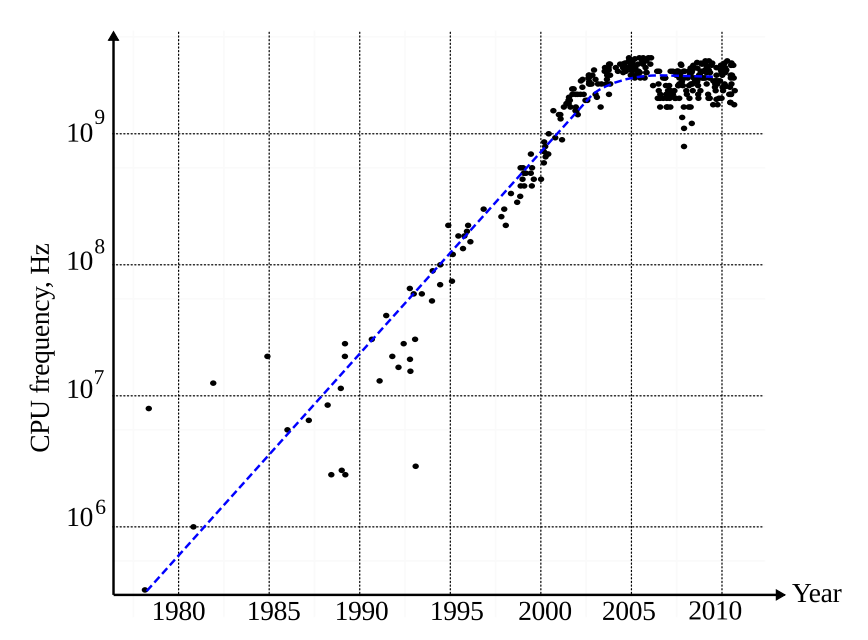
\includegraphics[scale=0.4]{../eldar_last_30_yrs}
	\caption[Frequency of the Intel microprocessors over past 30 years]{Frequency of the Intel microprocessors over past 30 years \cite{zianbetov2013phd}.}
	\label{fig:eldar_last_30_yrs}
\end{figure}\\
This plateauing of clock frequency has been caused by high power consumption, due to the demands placed by the global distribution of a high frequency clock, often the single biggest consumer of power on the chip \cite{tiwari1998reducing}.
With the growth of the \ac{IOT} market where low power devices are essential, with many of the emerging uses of \acp{SOC} being portable and thus without a permanent power source, high power consumption goes directly against one of the key pillars of the technology. This forces many of these devices to use lower performance hardware in order to reduce the power consumption, and increase their battery life,.

In digital systems, two main approaches are used when designing the clocking system. In both cases, the chip is broken down into small areas in which all transistors are clocked synchronously, with the size constrained by the ability to deliver a quality clock signal to all transistors. The first of these methods is \ac{GSLS}, where the clock signals in each of these subregions of the chip are synchronised with one other. In practice, however, this is very difficult to achieve, as extremely high precision is required across the ever increasing number of transistors and the entire area of the chip, and doing so leads to high power consumption.

In contrast, in \iac{GALS} clock delivery system the ``local'' areas are not synchronised with each other. This reduces the clocking system's complexity and thus the power consumption and chip area used, at the expense of communication speed between blocks. This disadvantage comes from the need to then somehow synchronise the messages being sent from one area to another to avoid message corruption.
\Iac{GSLS}, system, however, has the advantages of deterministic behaviour and greater rates of communication between clocking areas and, as such, remains a desirable system design. A number of methods which deliver \ac{GSLS} clocking exist at present, such as clock trees, as well as emerging technologies like the ADPLL network.

\section{The Impact of Clocking Errors}
In Figure \ref{fig:eldar_why_precise_clocking} the data path between two synchronously clocked registers is shown, with the circuit's function being carried out by the combinatorial network between the registers.
Each register has a setup time, which represents the amount of time that the input value to a register must remain constant before the clock edge, and a hold time, the time for which the input must remain constant after a clock edge.
\begin{figure}[h]
	\centering
	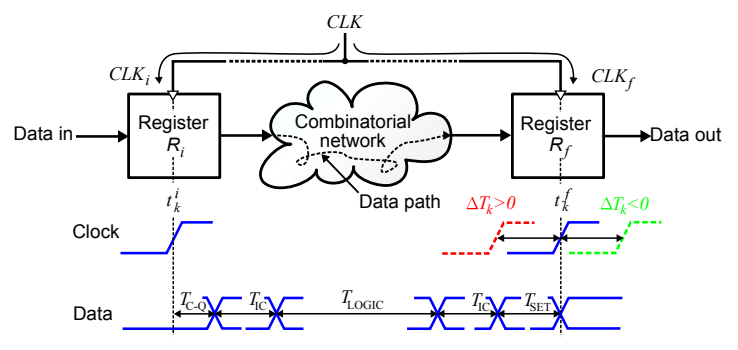
\includegraphics[scale=0.6]{../eldar_why_precise_clocking}
	\caption[Data flow in a clocked system]{Data flow in a clocked system \cite{zianbetov2013phd}.}
	\label{fig:eldar_why_precise_clocking}
\end{figure}

A lack of synchronisation between the clock edges will manifest itself as a time difference between the clocking events at both registers, $\Delta T = t^i_k - t^f_k$. $\Delta T$ is considered to be ergodic and can be described by an average deviation called skew and random process called jitter, normally modelled as a Gaussian random variable. If $\Delta T$ is negative, this reduces the time available for the intervening combinatorial network, thereby having the same effect as a reduction in clocking frequency. Correspondingly a positive $\Delta T$ for depicted registers implies a negative $\Delta T$ for $R_f$ and the subsequent register. 
The most common sources of clock error are caused by mismatches which usually stem from production, such as differences in the length of clocking paths, buffer delays or in the parameters of either active or passive components in the clock distribution network. As the size of components on \iac{IC} reduces, this mismatch becomes more difficult to avoid. All sources of mismatch will manifest themselves in the clock distribution system as skew between transistors, while the noise in active components or the power supply system will appear as jitter in the clock signal.

\section{Traditional Solutions}
A number of traditional solutions exist that produce \ac{GSLS} clocking systems, using a variety of techniques. The most simple of these implement clock distribution systems that are symmetrical in order to distribute a centrally generated clock signal to all areas of the chip at the same phase. These systems are named in accordance with their geometry, with the most common variants being branch, X or H trees. 
\begin{figure}[h]
	\centering
	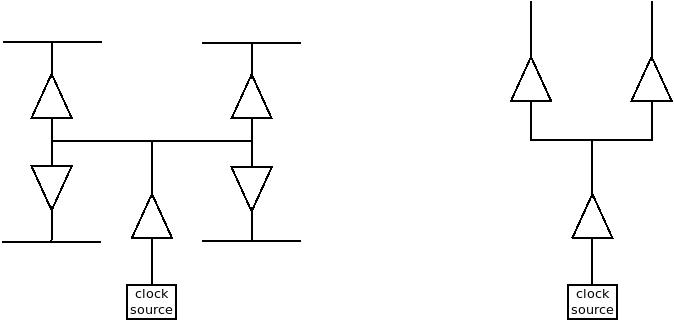
\includegraphics[scale=0.33]{../trees}
	\caption[H and branch tree clock distribution systems]{H and branch tree clock distribution systems.}
	\label{fig:trees}
\end{figure}

While on the surface these appear simple, the task of obtaining an exact matching is, in practice, the limiting factor in this design. Even if the clock distribution system is geometrically symmetrical by design, production mismatches in either active or passive components will lead to a skew that varies from part to part. In order to minimise the impact of production tolerances, the dimensions of components in the distribution network can be increased, thus reducing the relative variation possible. However this has the impact of increasing the power consumption of the distribution network \cite{tiwari1998reducing}.

A mesh clock distribution network, as in Figure \ref{fig:mesh} is an alternate design where the clock is delivered using a Cartesian grid of distribution lines. Compared to a tree type system, the variation in skew seen with a clock mesh, is inversely proportional to the density of the grid while the sources of jitter remain identical. According to Abdelhadi \textit{et al} (2010) clock meshes ``\textit{achieve low and deterministic skew, low skew variations, and low jitter}''; all desirable characteristics for a clock distribution system. However, they dissipate more power due to extra capacitive loading, attributable to the vast number of lines required to form the grid. Similarly, mesh distribution networks suffer from potential mismatch in production and alleviation, through increasing of the dimensions of interconnects, will, as with a tree type system, lead to higher power consumption \cite{abdelhadi2010timing}. 
\begin{figure}[h]
	\centering
	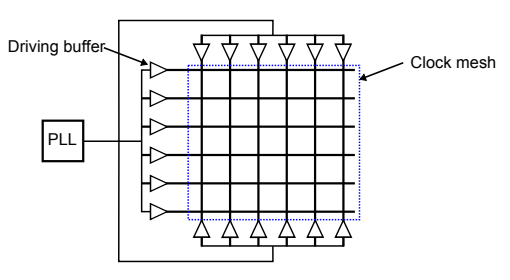
\includegraphics[scale=0.7]{../tex_files/eldar_mesh}
	\caption[Mesh clock distribution system ]{Mesh clock distribution system \cite{zianbetov2013phd}.}
	\label{fig:mesh}
\end{figure}

Alternative designs replace the electrical lines used in the tree networks with waveguides for optical signals, with only the distribution in the local area carried out using regular wires. This technique presents many advantages \cite{chen2006chip}: optical clock delivery is immune to the noise sources that affect electrical clock distribution systems, consume less power and do not suffer from the electrical losses present in a regular tree system. However, this is a fledgling method, and sufficient research into materials and potential designs has yet to be carried out \ref{zianbetov2013phd,1648640}.

\section{Skew Compensation}
In a tree type distribution system, skew is the main issue affecting clock accuracy and as such some effort has gone into addressing the problem. Skew due to the manufacturing process can be, at least, partly accounted for by means of active control through a skew compensator. This is a circuit, or controller, that compares the skew of each local clocking area on the chip and attempts to ensure in-phase clock delivery. Two main strategies exist to provide skew compensation, each named according to the location of the control mechanism. Designs featuring the controller located at the clock source, are known as ``centralised'' methods, and those with multiple controllers in the individual clocking areas are known as ``decentralised''. Regardless of the controller placement, these techniques allow for the tuning of the propagation delay between the centralised clock source and the local clocking areas.

In a centralised skew compensation circuit, the skew across the chip is calculated by the central controller, which then manipulates the distribution network in order to deliver a more in-phase clock around the chip. This calculation is done by measuring the round trip time from the clock source to both the root of the local clock tree, and to the individual ``leaves'' of the tree. The controller then has a limited ability to tune the propagation path. The downsides of this technique are that the resolution of both the measurement and compensation are poor, not permitting more than the correction of skew, and not of any jitter that may be present in the system. The extra circuitry required for both the tunability of the forward path, and the two extra return paths contributes to the increased footprint and power consumption of the distribution system.

As the name suggests a decentralised skew compensation technique, delegates the responsibility of tuning the propagation path to the individual clock regions. This strategy has the advantage of not requiring the return paths present in a ``centralised'' design. Instead, comparison is made between the leaves of different clocking areas and, on this basis, the propagation delay is varied.
For example, Yamashita \textit{et al} (2005) designed a system in which each clocking area or ``leaf node'' contains a partial clock tree. Each of these ``leaves'' is able to compare its clock phase to the neighbouring node, and based on the result, tune an adjustable delay buffer \cite{yamashita2005dynamic}. While this method can compensate for process, voltage and temperature variation, it does not address the power consumption due to the delivery of a high frequency clock across the entire chip area nor does it have any impact on clock jitter.

\section{Multi-oscillator Designs}
The designs described previously are similar, in that they have a single central oscillator that provides the clock for all areas of the chip, whereas the following methods attempt to synchronise multiple oscillators, each of which provides the clock for its own clocking area. The main advantages of a multi-oscillator design are that as each clocking area has its clock created locally, there is no degradation in the quality of the signal as it is distributed around the chip and the number of potential noise sources is reduced. In order to obtain global synchronisation some method of comparison between local clocking areas is required, and how this is done depends on the architecture. Regardless of how the comparison is made, it is carried out between neighbouring clocking areas and, therefore, the feedback network need not have a large footprint or power overhead.

One such method is a network of oscillators as in Figure \ref{fig:mizuno1998noise} which uses coupled \ac{PLL} to generate local clocks. Here the output of a leaf node is compared with an external reference and the operating frequency of each \ac{VCO} tuned based on the result.
\begin{figure}[h]
	\centering
	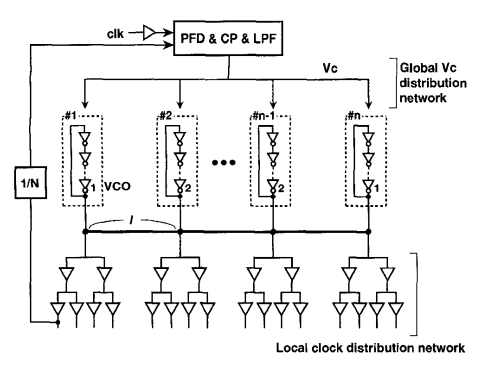
\includegraphics[scale=0.7]{../mizuno1998noise}
	\caption[Coupled oscillator clock delivery circuit]{Coupled oscillator clock delivery circuit \cite{mizuno1998noise}.}
	\label{fig:mizuno1998noise}
\end{figure}
The advantage of this method is the simplicity of the feedback network, requiring just the divided clock output from a single leaf node. The \acp{VCO} are then adjusted by the control voltage, $v_c$, which needs delivery to all areas of the chip. However, this is not a clock signal so does not suffer from skew or jitter. This alleviates the need for a power hungry distribution circuit, while also being more noise-immune than the transmission of a high frequency clock. This design does still suffer from clock variation as all \acp{VCO} are fed the same control voltage, and thus the manufacturing tolerance issues present in conventional designs persist here also. This is acknowledged by the authors:
\begin{quotation}
	\textit{Unfortunately, as with the conventional ... method, distributing the \acp{VCO} over the entire chip causes the problem that jitter and skew are increased by variations in the fabrication process (static), temperature, and power supply (dynamic)} \cite{mizuno1998noise}.
\end{quotation}
This type of multi-oscillator design is implemented by analogue circuits, and as a result not only the clock signals, but also the control signals are liable to variation due to noise, fabrication mismatch and power supply dynamics.

Another potential multi-oscillator clock distribution system uses the phase relationship between the oscillators driving neighbouring clock areas, in order to obtain synchronisation. Once again, this negates the requirement for a global distribution structure and the signals used for comparisons need only be sent between neighbouring clocking areas. As \iac{PLL} is being used, it is again possible to perform the phase comparisons using a divided version of the generated clock. This in turn means the hardware transporting the divided clock signal to the phase comparator, has significantly lower requirements placed on it, thus lowering the power consumption due to electrical losses. Pratt and Nguyen initially addressed this method of clock distribution in their 1995 paper entitled ``\textit{Distributed Synchronous Clocking}'' in which they proposed a Cartesian grid of clocking areas, each with their own \ac{PLL} This distribution method is known as \iac{PLL} Network \cite{pratt1995distributed}. In this design any given node is synchronised with its neighbours and one of the corner nodes is additionally synchronised with the reference. According to the authors, this is ``a simple, effective way to achieve low cost, high quality, low skew clock generation in a synchronous parallel processor''. They did, however, note the presence of a phenomenon called ``mode locking'', which is the settling of the network into a stable equilibrium where there are non-zero relative phases.

\begin{figure}[h]
	\centering
	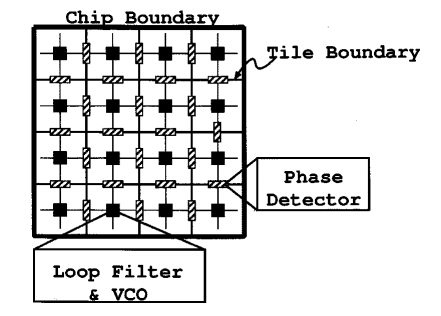
\includegraphics[scale=0.7]{../gutnik2000active}
	\caption[PLL network topology ]{PLL network topology \cite{gutnik2000active}.}
	\label{fig:gutnik2000active}
\end{figure}

This architecture of clock distribution network was then implemented by Gutnik \textit{et al} (2000) who fabricated a 4x4 array of oscillators, operating at a centre frequency of 1.2 MHz. The oscillator was implemented as a voltage controlled ``nMOS-loaded differential ring oscillator'', and in order to avoid mode locking the phase detector was implemented as a highly non-linear circuit. The design was a success and the authors concluded:
\begin{quote}
	\textit{Design and measurements on this chip confirm that generating and synchronizing multiple clocks on chip is feasible. Neither the power nor the area overhead of multiple \acsp{PLL} is substantial compared to the cost of distributing the clock by conventional means} \cite{gutnik2000active}.
\end{quote}

The remaining benefits of such a clock distribution system are: as the individual oscillators have their own control signal, mismatch between different oscillators is not a factor, as they will also receive different control signals. Secondly, and unlike the conventional methods, sources of jitter in the system, for example power supply dynamics, can be accounted for. Finally, symmetry between the different oscillators is not required, again attributable to the individual control signals in use. 

\section{ADPLL Networks}
As \iac{PLL} network is an analogue circuit, its integration in a modern \ac{IC} is a barrier to usage, and, therefore, it has not been used in any commercial designs \cite{zianbetov2013distributed}. An alternative design that is more suitable for current fabrication techniques, eschews from using analogue components and, instead, implements the network of controlled oscillators using only digital circuitry, hence the name All-Digital \ac{PLL}. A 4x4 \ac{ADPLL} network was designed and prototyped in 65 nm CMOS by Zianbetov and Shan in order to test the suitability of the technique as a clock distributor \cite{zianbetov2013phd,shan2014phd}.

In this design, the oscillators are once again laid out in a Cartesian grid, with each node phase coupled to their neighbours. As this is now a digital system, the coupling is carried out using digital phase comparators, which attempt to measure the phase difference between two oscillators. Figure \ref{fig:eldar_node} shows high level detail of the architecture of both the entire clocking system and that of an individual node in the design. The digital nature of this architecture brings with it a number of advantages over traditional analogue implementations, as it can benefit from advancements in digital circuit design suites, be reconfigurable and programmable, and has a significantly greater immunity to perturbations inherent to its digital nature, as the exact voltage of signals is of no importance \cite{zianbetov2013phd}. 

This last advantage is particularly useful in a digital environment, as otherwise there is potential for clock degradation resulting from switching of transistors. The drawback of the switch to a digital architecture, however, is the presence of quantisation. Analogue designs both deliver continuous control signals to the oscillators and have a continuous phase detection capability, unlike a digital system where these actions are carried out with fixed resolution.
\begin{figure}[!h]
	\centering
	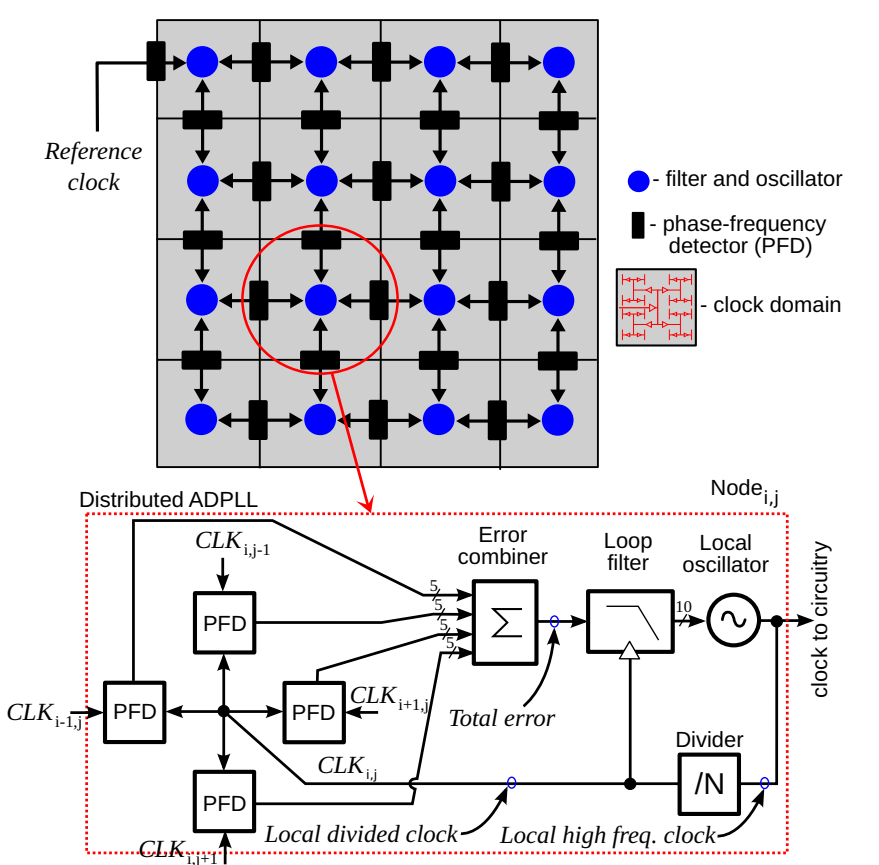
\includegraphics[scale=0.4]{../ccirc_2013_arch}
	\caption[Architecture of the ADPLL network and of a single node]{Architecture of the ADPLL network and of a single node \cite{zianbetov2013distributed}.}
	\label{fig:eldar_node}
\end{figure}
Looking at the design of a given node, it is notable that the function carried out by the Error Combiner is akin to an average, therefore as mentioned by Pratt and Nyugen, there is potential for a mode locked equilibrium in which the oscillators are not synchronised. In their paper, they presented a method where initial start-up was performed uni-directionally and, once all nodes are close to alignment, full connectivity could be restored, however this was not viable in an analogue system as reconfigurability was not an option \cite{pratt1995distributed}. Javidan \textit{et al} (2011) found that this was in fact the case, and stated:
\begin{quote}
	[Mode-locking] is solved in a simple and original way, by a dynamic reconfiguration of the network interconnection topology at the starting stage.
\end{quote}
In creating an entirely digital system, Zianbetov and Shan could easily reconfigure the network topology and, by implementing a uni-directional start-up, avoid the problem of convergence into a mode locked state, without having to design a non-linear phase detector.

\section{\acs{ADPLL} Architecture}
As indicated in Figure \ref{fig:mulkeen_pll}, the three main building blocks of a conventional \ac{PLL} are the \ac{PD}, \ac{LF} and \ac{VCO}. In \iac{ADPLL} these blocks are then replaced by their digital counterparts, necessitating quantisation in order to remain physically realisable. The ``All-Digital'' moniker is a misnomer as the oscillator and \acl{PD} are usually both implemented by mixed signal circuits.
\begin{figure}[h]
	\centering
	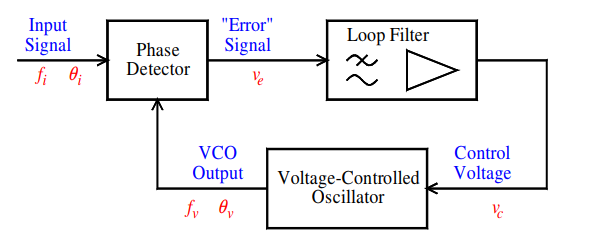
\includegraphics[scale=0.5]{../tex_files/mulkeen_pll}
	\caption[Block diagram of \iacl{PLL}]{Block diagram of \iacl{PLL}, \textit{Wireless Systems Notes}, B. Mulkeen (2017).}
	\label{fig:mulkeen_pll}
\end{figure}

\subsection{Digitally Controlled Oscillator}
In a digital system there are a very limited number of voltages representable, most commonly just two, so using a voltage to control the oscillator is not a viable strategy. Instead a fixed bit width signal is used to control the oscillator's period, selecting the number of inverters in a ring oscillator or the varactor configuration of a travelling wave oscillator \cite{chen2011rotary}. The decisions made in the design of the \ac{DCO}, or \ac{NCO}, determine many of the other \ac{ADPLL} parameters. While tuning range and centre frequency, as well as linearity, carry over from the analogue counterpart, \iac{DCO} also has a frequency step, which in combination with the bit width of the control signal determines the range over which the oscillator can be tuned. Figure \ref{fig:my_ring} illustrates a basic ring oscillator design. A ring oscillator is an inherently unstable circuit, composed of an odd number of inverters connected in a circle, which allows a signal to propagate infinitely, with the signal at any point in the circuit appearing as a square wave. The half-period of this oscillator is the time taken for the signal to propagate once through the chain, $n$ times the propagation delay through one inverter, where $n$ is the number of inverters. The frequency of operation can then be set by modulating the length of the chain, in steps of two inverters to maintain an odd number, by means of a control signal. The main impact of output frequency quantisation is that only frequencies which are at integer multiples of the frequency step away from the centre frequency can be easily reproduced. Intermediate values only obtainable in a manner akin to Fractional-N synthesis, with the control code toggling back and forth. This acts as a source of jitter in the system.
\begin{figure}[h]
	\centering
	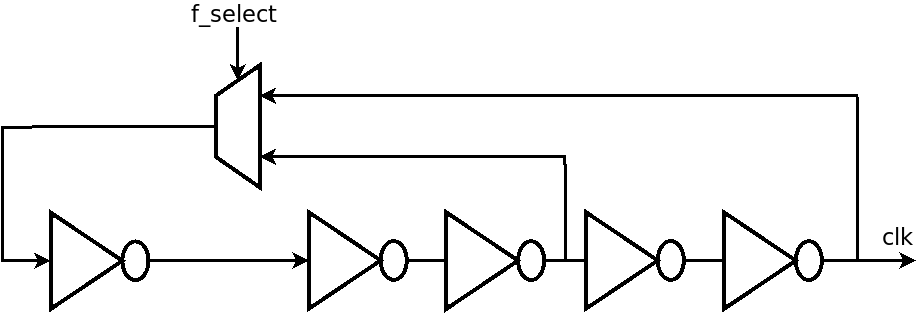
\includegraphics[width=0.6\textwidth]{../inverter_chain}
	\caption[Basic Ring/Inverter Chain Oscillator]{Basic ring/inverter chain oscillator.}
	\label{fig:my_ring}
\end{figure}

It is also possible to implement \iac{NCO} by means of a counter, in a manner that will produce either linear period or linear frequency steps. Both methods use the most significant bit of the counter's value to form the output signal. Period linearity is achieved by varying the reload value of the counter after overflow, depending on the control code, thereby changing the period by a multiple of a fixed step. Alternatively, frequency linearity can be achieved if the reload value is left constant, but instead the amount added to the counter every clock cycle is changed according to the control code, once again a fixed step size is used.

\subsection{Digital Phase Detector}
Once again quantisation impacts the \acl{PD}, as rather than a continuous output, the phase detector in \iac{ADPLL} has a finite number of output values, thus limiting the accuracy of the phase detector. A second form of quantisation is also present, as unlike an analog system, a digital phase detector does not provide continuous data in the time domain, instead relying on sampling. At its most basic, a digital phase comparator may only output an indication of which signal is leading, a design known as a Bang-Bang Detector. This can be constructed using a single D Flip Flop, with the generated signal connected to the ``D'' input and the reference signal acting as the clock. As the output only has two levels, the resultant word is only 1 bit wide, limiting the range over which the output frequency can be controlled. More complex designs, such as that in Figure \ref{fig:shan_bb_pd} implemented by Shan, build on this by measuring the time difference between edges of the signals using \iac{TDC}, in his case using \iac{TDL} \cite{shan2014phd}. \Iac{TDL} is constructed by a chain of elements of a fixed delay, and the signal to be timed is applied to this start of this chain. After the timing interval elapses the values at each point in the chain are examined, and using temperature coding, these are converted to a digital signal. The width of this signal is the bit width of the \ac{PD}'s error signal. This mimics a time measurement and allows for the phase difference to be recorded in a non binary manner.

\begin{figure}[h]
	\centering
	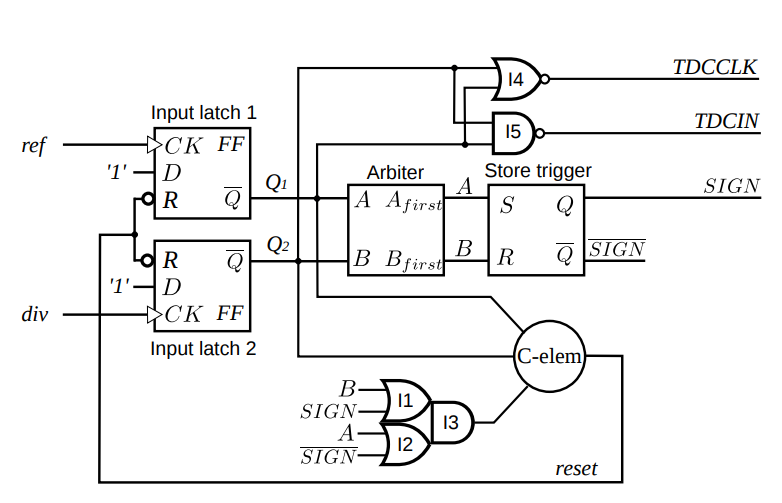
\includegraphics[width=0.65\textwidth]{../shan_bb_pd}
	\caption[Bang-bang phase/frequency detector architecture]{Bang-bang phase/frequency detector architecture \cite{shan2014phd}.}
	\label{fig:shan_bb_pd}
\end{figure}

\subsection{Digital Loop Filter}
\begin{figure}[h]
	\centering
	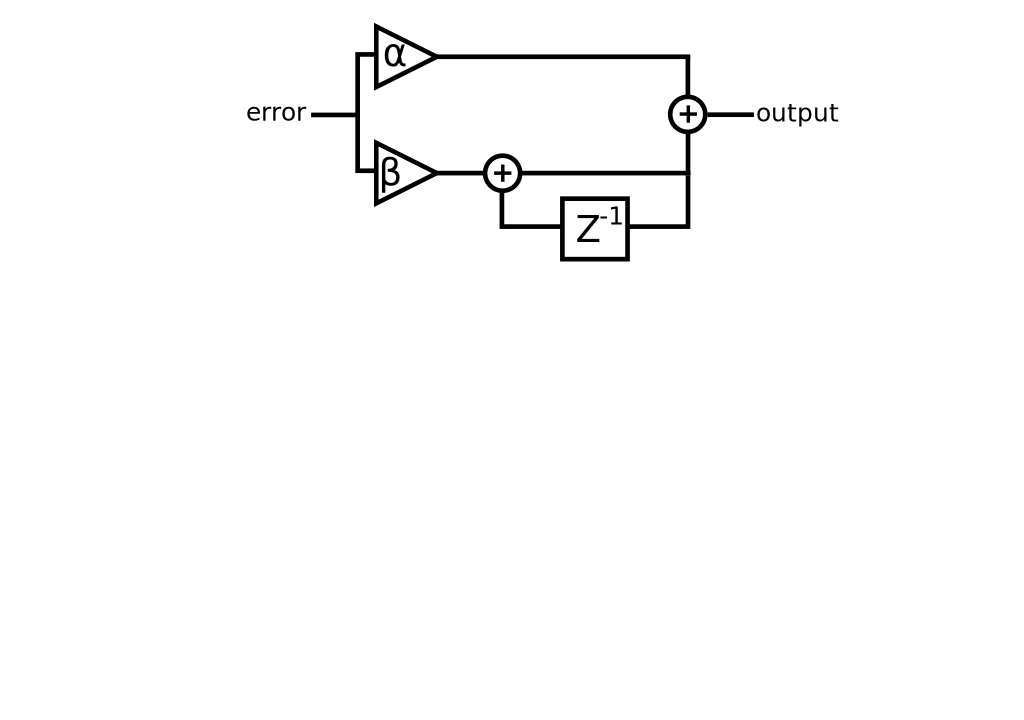
\includegraphics[width=0.6\textwidth]{../simple_pi}
	\caption[Basic \ac{PI} controller architecture]{Basic \ac{PI} controller architecture.}
	\label{fig:my_simple_pi}
\end{figure}
The \acl{LF} in \iac{ADPLL} can be implemented as \iac{PI} controller, as only a low-pass filter is required, such as that in Figure \ref{fig:my_simple_pi}. In the case of a node in \iac{ADPLL} network the input of this filter is a weighted average of the phase difference relative to the neighbouring local clocking areas. In a digital system, the proportional section can be implemented by a simple multiplier, whereas the integral path is constructed by the delayed addition of error multiplied by the integral gain to the sum of past values. This delayed accumulation can be easily implemented by an accumulator to which the current value of the multiplication is added each cycle, and as a result the system has an infinite impulse response. The value of these gains determine the response and stability of the \ac{ADPLL} network. The transfer function of such a controller is given by \cite{shan2014phd}:
\begin{equation*}
	H(z) = \alpha + \beta\frac{1}{1-z^{-1}} = \frac{(\alpha + \beta) - \alpha z^{-1}}{1-z^{-1}}\vspace{-0.2cm}
\end{equation*}
It has been found by Koskin \textit{et al} (2018), that stable operation can be achieved when the integral gain, $k_i$, is less than half the proportional gain, $k_p$ \cite{koskin2018generation}. In the same study a range of values was found which would produce low jitter operation of the network. As these values are all less than one, the filter must implement fixed point arithmetic in an effort to maintain the simplicity of the \ac{LF}, rather than incurring the penalty of floating point calculations.

\subsection{Error Combiner}
The \acp{ADPLL} used in a network need to combine the error signals from multiple neighbours to determine what the average difference from its neighbours is, and this necessitates the addition of an Error Combiner. In a digital system, this can be implemented by a weighted average of the different error signals, with the weight being modifiable at run-time. This configurability is what permits the system to implement uni-directional mode and also allows for the weighting applied to certain signals, such as the external reference, to be modified. The ease of implementation of a configurable error combiner is one of the key advantages of \iac{ADPLL} over an analogue system.

\section{The Role of the FPGA}
\Iacl{FPGA} is a type of \ac{IC} that is designed to be configured by a designer after the chip itself has been manufactured. \Iac{FPGA} contains a large number of logic elements that can be connected together in order to perform complex logic, written using the same \aclp{HDL} (\acsp{HDL}) used to design the digital blocks of \aclp{ASIC} (\acsp{ASIC}). They may also implement standard modules such as adders, multiplexers and \ac{RAM} as a fundamental element. More complex logic is often implemented using multiplexed lookup tables rather than true logic elements. High end devices such as the Xilinx Zynq Ultrascale, may implement Multi-Processor \ac{SOC}s. Compared to \iac{ASIC} the designer does not have direct control over the layout of the system but rather describes its behaviour, possibly down to the basic logic elements of inverters or other gates. Limited control is possible over the placement of the individual modules, but \ac{EDA} tools are responsible for the exact placement of elements. As a result, it is not possible to have precise control over the delays experienced as signals propagate through the design. To assist with the resolution of any issues \ac{EDA}s provide tools to analyse timing behaviour.

Prototyping on \iac{FPGA} is a common verification stage for conventional \ac{ASIC} designs, as it allows for a hardware validation of any digital circuitry, and the detection of any potential flaws or errors made by the design before the expense of \iac{ASIC} implementation. In their 2013 \ac{ADPLL} network implementation, Zianbetov and Shan used \iac{FPGA} in order to validate their programming interface, the design of the error processing block, ensure they had eliminated mode locking behaviour and to ensure phase synchronisation was possible \cite{zianbetov2013phd,shan2014phd}. However they experienced two main limitations: they were not able to implement the mixed-signal \ac{PFD} and \ac{DCO}. Secondly, the maximum frequency of operation possible was orders of magnitude lower than the GHz range of their \ac{ASIC} implementation. These issues were circumvented by implementing an alternative \ac{PFD} and \ac{DCO} designs which were driven by the clock distribution network provided by the \ac{FPGA}, and frequency scaling each clock by the same amount, such that the results of testing would remain indicative. One of the main advantages they saw was that the hardware description used for the digital blocks of their \ac{ASIC} could be directly ported over to the \ac{FPGA}.

A similar technique was used by Lata \textit{et al} (2013) to implement \iac{FPGA} clocked oscillator with a $200~\si{\kilo\hertz}$ centre frequency, however it is hard to understand exactly what either the goal was or the specifics of the \ac{DCO} used \cite{lata2013adpll}.

It is possible to implement limited mixed-signal circuits on \iac{FPGA} through the use of primitive logic elements, however, as control over the implementation is restricted to the module level, it is not possible to mirror the implementation of a design intended for \iac{ASIC}. As these implementations are analogous to a mixed-signal circuit on \iac{ASIC}, the verification of theoretical behaviours, as done by Koskin \textit{et al}, in order to test the findings of his PhD thesis \cite{theboys2019}, is made possible without the expense of \ac{ASIC} fabrication. \Iac{FPGA} based mixed-signal \ac{ADPLL} network is also seeing use here in \ac{UCD} as a initial prototyping platform for the validation of new modules for use in \ac{ASIC} based \ac{ADPLL} networks.

\ac{FPGA}s have been used in other fields to simulate and experiment with new technologies, although not all of these attempt to implement the mixed-signal circuitry using primitive elements. Fernandez-Alvarez \textit{et al} (2016) proposed a method for prototyping high-voltage system controllers suited to higher end \ac{FPGA}s in which a co-processor on the \ac{FPGA} simulates the mixed-signal circuitry while the digital section of the design is implemented on the \ac{FPGA} itself \cite{fernandez2017hw}. While the interfacing between hardware and software remains a challenge they found:
\begin{quotation}
	Obtained data are compared to the data obtained by means of using ... simulation. The proposed solution speeds up the evaluation in around one order of magnitude keeping the accuracy. The output signal differs in less than 0.6 mV (RMSD).
\end{quotation}

Mixed-signal circuits were, however, simulated in hardware by \'{O}scar Luc\'{i}a \textit{et al} (2011) on \iac{FPGA}, in order to overcome the excessive time penalty imposed by software based simulations that required the behaviour of both a digital and mixed-signal peripheral and that of a microcontroller running code in C to be simulated side by side \cite{lucia2011real}. They concluded
\begin{quotation}
	... the proposed system provides a versatile and fast method to develop ad hoc control architectures, avoiding the need for time-consuming mixed-signal simulations and the risk of damaging the actual power converter implementation.
\end{quotation}
By carrying out simulations on \iac{FPGA}, Guanhua Wang \textit{et al} (2013) achieved a 3000 times decrease in run-time when compared to an identical simulation in MATLAB used for the verification of a calibration algorithm for successive approximation analogue-to-digital converters \cite{wang2013fast}. Many other examples can be found of \ac{FPGA}s used for the simulation of mixed-signal or \acs{RF} circuits.
%TODO Elena had suggestions?

\section{\acs{ADPLL} Performance Characterisation}
As already stated, the goal of a clock distribution system is to synchronise clocking events in all areas of the chip. The effectiveness of this synchronisation is characterised by two main metrics, jitter and skew, which together describe the distribution of clocking events. Skew is the average time delay between a clocking event in one area of the chip and that of a reference event. It can be easily measured by computing the average value of this delay. Jitter has a number of definitions depending on how it is measured, but at its most basic, it is the standard deviation of the time delays with respect to the reference clocking edge.

The simplest form of clock performance characterisation is on \iac{C2C} basis, in which the reference is the previous edge of the signal under test itself. Here the standard deviation of the individual delays gives the jitter of the signal. As the previous edge of the generated signal is used as the reference, and thereby the delay is the period of the signal, the mean value is no longer the skew, but instead can be used to compute the centre frequency over the time interval. For a more informative measurement the \ac{TIE} can be computed, which takes into account another signal as the reference. \ac{TIE} is calculated by comparing the delay between the signal in question and a reference that is treated as ideal. The mean value gives the relative skew between the two signals and, once more, the standard deviation of the measurements gives the jitter with respect to this reference.

Both above forms of measurement assume a large number of sequential measurements, however, there are other ways that jitter and skew can be calculated \cite{AN10007}. Phase jitter is an important characteristic for communications systems as it can be used to calculate phase noise, important to ensure spurious emissions are within legal requirements. Long term, or accumulated, jitter represents the cumulative effect of jitter on the signal over several cycles. Long term jitter in particular affects \acs*{RADAR} as it will manifest itself as a Doppler shift in the return signal. For \iac{PLL} network, with an appropriately designed filter, the long term jitter should be zero so long as the reference signal is stable. %TODO ask Brian about this one

\setcounter{chapter}{2}

\chapter{ADPLL Designs for FPGAs}\label{chap:3}

\section{Chapter Overview}
The first step in creating an \ac{FPGA} based network of \ac{ADPLL}s is the design of the \ac{ADPLL} itself, which will be addressed in this chapter. The nature of an \ac{FPGA} necessitates a number of compromises in the design of a given block which limits transferability to \ac{ASIC} designs. In this chapter the potential designs for each individual block, or module, investigated will be explained and the case for their selection in an \ac{FPGA} based \ac{ADPLL} made. A number of blocks have implement purely digital circuitry and as such can be transferred in their entirety from an \ac{FPGA} and vice versa. However, those that will be used to emulate mixed-signal circuitry, such as the \ac{DCO} and \ac{PFD}, will be examined in greater detail.

\section{Digitally Controlled Oscillators}
The choices made in the design of the \ac{DCO} have the greatest impact on the effectiveness of the overall platform and which use cases the \ac{ADPLL} containing it are suitable for, as the key performance benchmarks are all done using the waveform this block generates. This project will address three distinct designs of \ac{ADPLL}s suitable for implementation on an FPGA, two derived from the clocks generated by the \ac{FPGA}s own distribution network and one generated independently of this clock, using a chain of inverters. These are not the only ways in which an oscillator could be synthesised on an \ac{FPGA}, however other designs were deemed to be unsuitable for extensible and portable implementations.

A prime example of this is the use of Xilinx proprietary \texttt{IODELAY} blocks to create an oscillator, as detailed in Xilinx Application Note XAPP872 \cite{iodelay}. The key idea here is that the bulk of the period is made up by the propagation time through one of the \texttt{IODELAY} blocks, which can be set at implementation time. This is combined with a section of an inverter chain, and a multiplexer used modify the length of this segment, the output of which is fed back into the \texttt{IODELAY} block. This method was discarded as the number of \texttt{IODELAY} blocks is very limited, so expanding to a larger network would be impossible, and they are all located around the edge of the chip, not suited to the construction of a Cartesian grid.

The main issue with the creation of \ac{DCO}s on an \ac{FPGA} is the inability to create mixed-signal circuits, such as those that would be intended for use on an \ac{ASIC}. As such the \ac{FPGA} based oscillator must emulate the behaviour of a mixed-signal circuit in some way.

\section{\acs{FPGA} Driven, Linear Period \acs{DCO}}
The first design of \ac{DCO} to be examined is of the type used by Zianbetov in his \ac{ADPLL} network test bed and relies on a counter driven by the clock manager on the \ac{FPGA} \cite{zianbetov2013phd}. At each event on the \ac{FPGA} provided clock a counter is incremented, overflowing upon increment past the maximum possible value. The \ac{MSB} of this counter forms the waveform generated by this oscillator, the period of which is controlled through an adjustable value that is loaded into the counter once overflow is reached, and forms the starting points for the counter. The period of oscillation is given by:
\begin{equation}
	T_{osc} = \big(2^{width} -~(BIAS+CC)~\big)\times T_{FPGA}
\end{equation}
where $T_{FPGA}$ is the clock period of the \ac{FPGA}, $CC$ is the control code input, $BIAS$ centres the oscillator in the middle of the tuning range in the event that the control code is zero and $width$ is the width of the counter used. As the only variable here is the control code, period step of this design is $T_{FPGA}$, thereby providing period linearity with respect to the control code. This is the key advantage of this design, as most \ac{ASIC} implementations of a \ac{DCO} are also linear in period. The other main reason to choose this design is that its \ac{FPGA} clocked nature allows for exact control over the frequency of operation, and the number of tunable parameters make it possible to configure multiple ways to achieve the same frequencies of operation. Combined these attributes make it very easy to create an oscillator that emulates the behaviour of a design intended for an \ac{ASIC}, however, at a greatly reduced frequency. This restriction on the frequency of operation arises out of the period step size, which in order to obtain a good resolution must be orders of magnitude smaller than the intended period to be generated. As the output waveform is taken from the counter's \ac{MSB}, the reload value of the counter must never go beyond $2^{width-1}$, as otherwise the output waveform will become a constant 1. As the reload value varies the low time of the \ac{MSB}, if the desired output waveform is a square wave this design will not be suitable.

In being \ac{FPGA} clocked this design has pseudo-deterministic characteristics, with each period step being almost identical across oscillators and over the entire tuning range, unlike an \ac{ASIC} where process variation will impact the layout of a high frequency oscillator. The only variation in this design will come, ironically, from jitter or skew in the \ac{FPGA}'s clock distribution network, which as the frequencies will typically be in the low hundreds of MHz is very minor. In the case of the Xilinx \acl{Nexys} this is at most 100 picoseconds, or 0.05\% of the period of an intended output clock at 5 MHz. To put this value into perspective, on this board the minimum value of $T_{FPGA}$ that could be used to drive this oscillator is 3.87 nanoseconds, 1.935\% of the period.

The resulting \ac{DCO} is best suited to applications that do not seek to gain a better understanding of oscillator performance, but rather those focused on validating the entirely digital blocks in the system, the role in which Zianbetov and Shan used this type of oscillator \cite{zianbetov2013phd,shan2014phd}.

\section{\acs{FPGA} Driven, Linear Frequency \acs{DCO}}
The second \ac{FPGA} clocked oscillator is similar in most attributes to the above design but eschews period linearity for frequency linearity. Again the overflow property of a counter is used with the counter's \ac{MSB} as output of the block, however, this time it forms a square wave. Rather than setting the reload value of the counter, instead the increment is adjusted depending on the control code, thus requiring $\frac{2^N}{BIAS+CC}$ increments to overflow. Accordingly the frequency of operation is set by:
\begin{equation}
	f_{osc} = f_{FPGA}\times\frac{BIAS+CC}{2^{width}}
\end{equation}
Here the control code $CC$ and bias are added to the value stored in the accumulator at each event of the \ac{FPGA}, clock until overflow is reached. This occurs at $2^{width}$ where, as before, $width$ is the bit width of the counter, thus valuing each control code increment at $\frac{f_{FPGA}}{2^{width}}$ Hz. As with the previous design, this oscillator is better suited to frequencies where the output of the \ac{DCO} is orders of magnitude lower than the clock signal driving it, as this ensures that the incremental change due to the control code remains a small fraction of the period.

This design is just as configurable as its linear-in-period counterpart, and well suited to the low frequency emulation of \ac{ASIC} based oscillators that are themselves linear in frequency. In sharing the \ac{FPGA} as a clock source again the pseudo-deterministic characteristics return, once more meaning this oscillator is better used for testing, simulating or verifying other blocks in the system.

\section{Inverter Ring \acs{DCO}}




\setcounter{chapter}{3}

\chapter{Network Implementation}\label{chap:4}

\section{Chapter Overview}
This chapter will cover the network implemented in the course of the project, beginning with the individual \ac{ADPLL}'s composition. A number of attributes for each design will be used to analyse and compare their performance. The impact of some minor architectural changes will also be covered, before the implementation of test network will be described. This chapter will also highlight some pitfalls encountered in the process. The \ac{HDL} Verilog was selected for use in this project due to my prior exposure to that language. 5 MHz was chosen as the target centre frequency for these \ac{ADPLL}s, during initial testing it was discovered that the waveform output via the Digilent Nexys4 development board's \ac{GPIO} ports began to degrade around the 10 MHz mark, preventing accurate analysis.

\section{\acs{ADPLL} Architectures}
Three different architectures of \ac{ADPLL} were implemented in this project for the purposes of testing, and re-use in the future within the research team in \acl{UCD}. Between each design a number of blocks remain constant, as only a single instance of that block was implemented, as variation its design would have negligible impact on the final system. These blocks were the error combiner and frequency divider. The loop filter was implemented both using fractional and integer arithmetic, but as the exact same calculation was performed in both cases there was no impact on the output of the module.

The three architectures chosen for implementation represent a progression from entirely an \ac{FPGA} clock driven system to an \ac{ADPLL} with all components asynchronous with respect to that clock. Therefore the first \ac{ADPLL} design features a clocked oscillator and phase detector, specifically the linear frequency design mentioned in Chapter \ref{chap:3} and the clocked phase detector using a state machine and a bi-directional counter. Skipping over Design 2, the final design used was asynchronous in totality, featuring the \acl{RO} and SigNum/\ac{TDL} phase detector. Design 2 sat between these two, using the \ac{RO} as its oscillator, but retained the clocked phase detector seen in Design 1.

The extensibility of the end product of this project was to the forefront during the design process. Whilst, apart from frequency, there were no guidelines as to what the system should resemble and a number of attributes could be chosen arbitrarily, a future user of this platform could have entirely different requirements or specifications. As such each block was implemented in such a way that changing the number of bits used for a certain signal, the target frequency or swapping between different blocks could be done with the sole requirement of changing Verilog \texttt{localparam}\footnote{A \texttt{localparam} is a constant that cannot be modified in a module instance statement \cite{hdlworks}}s in the module \footnote{Module is the Verilog term for a number of logic elements grouped to provide a certain functionality} in which change was made, which would then propagate to any sub-modules affected. Starting the design process with this in mind was a major benefit at later stages when frequent modifications were being made to test their impact, or when changing between \ac{ADPLL} designs.

\subsection{Generic Components}
As mentioned in the chapter overview, a number of components were used in all \ac{ADPLL}s implemented, as changes in their design would not impact the overall system.
\subsubsection{Error Combiner}
The error combiner in this design had a number of requirements in order to be suitable for use in both a single \ac{ADPLL} as well as a network operating in both uni- and bi-directional modes, alongside modifications which would change the widths of the error signals requiring averaging. The module was implemented on the basis that the \ac{LF} input width would be identical to the phase detector output width.

The error combiner was designed to take in up to four error signals, all of an identical width which defaults to eight, and four weights to apply in the summation process. A weighted summation is performed by multiplying each error signal by the weight and adding the results together. Regardless of the number of input error signals, a division by four is then performed in order to compute the average error, done by shifting the value right by two. In a \ac{HDL}, unlike C programming or similar, a shift requires no computation and is instead implemented by performing a part-selection. As all error signals are two's complemented signed integers, the error combination process is also carried out using signed values. The code implementing the error combiner can be found in \textsc{ErrorCombiner.v}, attached in Appendix \ref{adx:code} Listing \ref{lst:error_combiner}.

\subsubsection{Frequency Divider}
The frequency divider is implemented using ``Divider 2'' from Chapter \ref{chap:3}, as only divisions ratios of 2, 4 and 8 were selected for use in the testing process. For ease of testing, the divider had outputs representing each of these division ratios simultaneously, which could be multiplexed between at runtime if so desired. A fourth output passed the input through unmodified, allowing for the divider to be removed without regeneration of the \ac{FPGA} configuration.
\begin{figure}[h]%
	\centering
	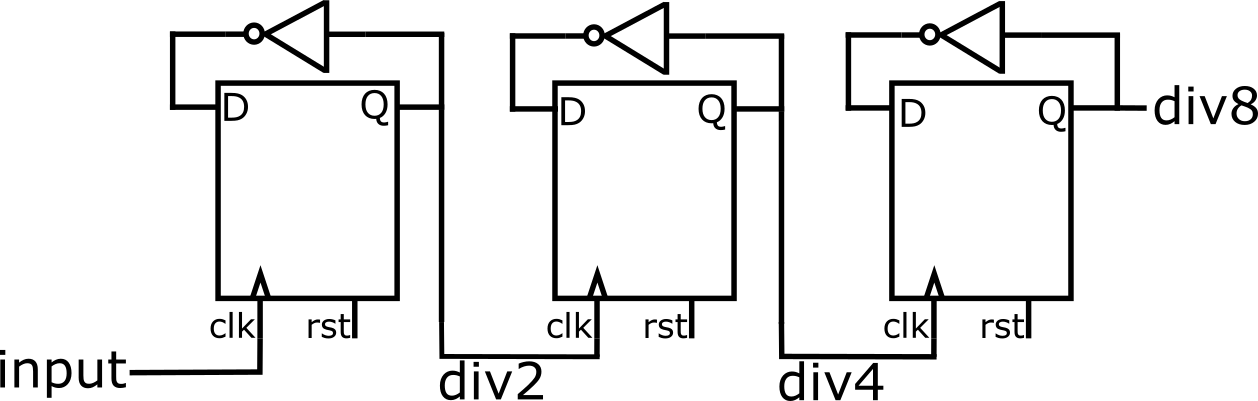
\includegraphics[width=0.6\textwidth]{../divider2}
	\caption[Frequency divider \ac{RTL} diagram]{Frequency divider \ac{RTL} diagram.}
	\label{fig:divs_impl}
\end{figure}

\subsubsection{Loop Filter}
Two \acl{LF}s were implemented, both as \ac{IIR} filters. \ac{FIR} was dismissed due to the extra hardware required to implement the calculations within a single clock cycle, as the \ac{LF} is clocked using the oscillator output, and the greater difficulty of gain adjustment compared to an \ac{IIR}. Clocking on using the generated signal ensures that the discrete time integration is only carried out once per phase comparison. A pitfall that may be encountered implementing an \ac{ADPLL} featuring a divider is not clocking the module on the divided clock, which will result in the integration being carried out at the oscillator output frequency.

Each of integer and fixed-point arithmetic were used to implement a filter respectively, however both designs are interchangeable as they perform the integration identically, given the same proportional and integral gains. All testing was carried out using integer arithmetic, as in Figure \ref{fig:integer_lf}, however the interchangeability will be confirmed later in this chapter, in Section \ref{section:minor_variations}. Additionally the \ac{LF} supports variation of both \acs{ki} and \acs{kp} at runtime, however, if a static value is desired the runtime variation may be disabled using a \texttt{parameter}\footnote{Parameters are constant values that may be changed at compile time, or in the module instance statement \cite{hdlworks2}}.
\begin{figure}[h]%
	\centering
	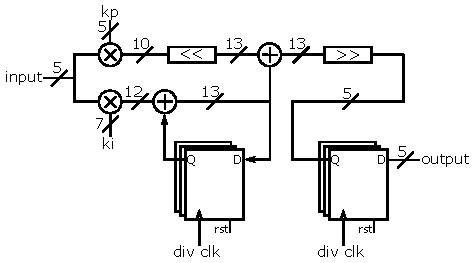
\includegraphics[width=0.8\textwidth]{../integer_lf} 
	\caption[\acl{LF} implemented using integer arithmetic \ac{RTL} diagram]{\acl{LF} implemented using integer arithmetic \ac{RTL} diagram (signal widths using default values).}
	\label{fig:integer_lf}
\end{figure}

Figure \ref{fig:integer_lf} contains an \ac{RTL} diagram describing the implementation. Important to note is the shift applied to the result of the multiplication by \acs{kp} which, as the integration is performed with a larger width to avoid accumulator overflow, preserves the intended relationship between proportional and integral gains.
The Verilog implementation of the \ac{LF} using integer arithmetic can be found in \textsc{LoopFilter.v}, attached in Appendix \ref{adx:code} Listing \ref{lst:loop_filter}.

\subsection{\acs{ADPLL} Design 1}
\acs{ADPLL} Design 1 is comprised of the aforementioned generic components and \ac{FPGA} clocked implementations of the \ac{PFD} and \ac{DCO}. This was the first solution addressed in the course of this project as it is the simplest to both implement and test, as all aspects of the \ac{ADPLL} are driven by the \ac{FPGA} clock. Compared to later designs utilising the \ac{RO}, Vivado simulations could be carried out, with accurate timing behaviour, depicting the locking process. The \ac{DCO} was chosen to be linear in frequency in order to obtain a square wave output as it was not yet known whether the varying pulse width of a period linear design would cause a problem in modules which, at that stage in the project, had not yet been designed. Indeed, a later discarded version of the \ac{FPGA} clocked \ac{PFD} relied on equal low and high times. The \ac{PFD} itself was implemented using a Moore type \ac{FSM} driving a up-down counter to convert the time between rising edges to a digital signal.

\subsubsection{\acl{DCO}}
As the \ac{FPGA} clocked, linear frequency oscillator is based on the use of counters, the first stage in its design was the decisions as to their required widths. The equation given previously is used here, with the control code set to zero in order to obtain the centre frequency, and 5 MHz as the target \ac{DCO} frequency:
\begin{align}
f_{osc} &= f_{FPGA}\times\frac{BIAS+CC}{2^{width}}\\
5\times 10^6 &= f_{FPGA}\times\frac{BIAS}{2^{width}}
\end{align}
This still leaves three parameters undecided: The \ac{FPGA} clock, the bit width of the counter and the bias point. As the \ac{FPGA} clock determines the frequency step of the design, a test counter was implemented initially to determine the maximum frequency at which the timing violations would not occur, at this was determined to be 275 MHz. The equation can then be updated, giving the relationship between bias point and counter width:
\begin{align}
5\times 10^6 &= f_{FPGA}\times\frac{BIAS}{2^{width}}\\
\frac{5}{275} &= \frac{BIAS}{2^{width}}
\end{align}
The maximum value of the counter must also be large enough such that with a bias point that allows for a reasonable range of frequency steps to be added or removed. 
This oscillator was originally designed to allow for 64 control codes either side of the bias, which called for a bias point of 65 or greater.
\begin{align}
\frac{5}{275} &= \frac{65}{2^{width}}\\
2^{width} &= \frac{65\cdot275}{5} = 3575 \\
width &= \left \lceil{\log_2 3575}\right \rceil = 12
\end{align}
From the above equation, the smallest counter that can satisfy this constraint is 12 bits wide, however when testing was carried out using a 275 MHz clock timing violations were discovered by Vivado, resulting \ac{FPGA} clock speed reduction to 258 MHz in order to resolve these violations. The correct bias point could then be calculated as $79$:
\begin{align}
\frac{5}{258} &= \frac{BIAS}{2^{12}}\\
 BIAS &= \left \lfloor{\frac{5\cdot 2^{12}}{258}}\right \rceil = \left \lfloor{\frac{20480}{258}}\right \rceil = 79
\end{align}
The frequency step can now be computed as all parameters have been chosen:
\begin{equation}
f_{step} = \frac{f_{FPGA}}{2^{12}} = 62.988~\si{\kilo\hertz}
\end{equation}
At the target frequency of 5 MHz this corresponds to a change in period of:
\begin{align}
f_{step0} &= 79 \times f_{step} = 79 \times 62.988~\si{\kilo\hertz} = 4.976~\si{\mega\hertz} \\
f_{step1} &= 80 \times f_{step} = 80 \times 62.988~\si{\kilo\hertz} = 5.039~\si{\mega\hertz} \\
T_{step}  &= \frac{1}{f_{step0}} - \frac{1}{f_{step1}} = \frac{1}{4.976\times 10^6} - \frac{1}{5.039\times 10^6} \\
T_{step}  &= 2.5~\si{\nano\second}
\end{align}
From the frequency step, control code range and bias the frequency range of this oscillator can be found:
\begin{align}
f_{osc} &= (BIAS+CC)\times f_{step} = (79+CC)\times 62.988~\si{\kilo\hertz}\\
f_{min} &= (79+CC_{min})\times 62.988~\si{\kilo\hertz} = (79-63)\times 62.988~\si{\kilo\hertz} = 1.008~\si{\mega\hertz}\\
f_{max} &= (79+CC_{max})\times 62.988~\si{\kilo\hertz} = (79+63)\times 62.988~\si{\kilo\hertz} = 8.944~\si{\mega\hertz}
\end{align}

Figure \ref{fig:osc2_impl} contains an \ac{RTL} diagram of this oscillator's implementation. As phase error is a two's complement signed value, its addition to the bias must be carried out using signed arithmetic. Provided the bias is greater than the minimum possible phase error, as has been ensured in this case, the result of this addition is positive signed integer. Being a positive quantity, additional logic performing a conversion from a signed to an unsigned representation is required.
\begin{figure}[h]%
	\centering
	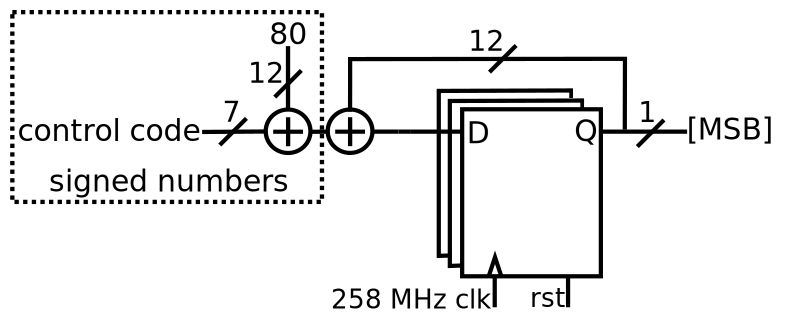
\includegraphics[width=0.8\textwidth]{../osc2_impl} 
	\caption[\ac{DCO} \ac{RTL} diagram as implemented]{\ac{DCO} \ac{RTL} diagram as implemented.}
	\label{fig:osc2_impl}
\end{figure}

\subsubsection{Phase Detector}
As previously mentioned the \ac{PFD} is also implemented using the \ac{FPGA} clocked approach, with sign detection carried out using a Moore Machine. The state transition diagram given as the example in Chapter \ref{chap:3} is that used to design this sign detector. The hardware description of this block is found in \textsc{PhaseDetector.v}, attached in Appendix \ref{adx:code} Listing \ref{lst:PhaseDetector}.
\begin{figure}[h]
	\centering
	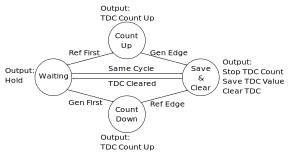
\includegraphics[width=0.8\textwidth]{../state_trans_new}
	\caption[Example State Transition Diagram for a Moore Machine]{Example State Transition Diagram for a Moore Machine.}
	\label{fig:state_trans_reprint}
\end{figure}

The synchroniser circuits are implemented by a pair of ``D'' flip-flips connected in series, clocked on the \ac{FPGA} clock. This synchroniser works by assuming that metastability will only persist for the duration of one \ac{FPGA} clock cycle as depicted in Figure \ref{fig:synchroniser_behav}. In the case where only one clock signal may experience metastability, two synchronisers are required in order to maintain symmetry in the phase comparison.
\begin{figure}[h]
\centering
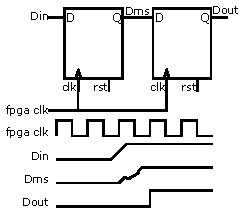
\includegraphics[width=0.4\textwidth]{../synchroniser_behav}
\caption[Double ``D'' flip-flip synchroniser circuit \ac{RTL} diagram]{Double ``D'' flip-flip synchroniser circuit \ac{RTL} diagram.}
\label{fig:synchroniser_behav}
\end{figure}

This \ac{FSM} then controls an Up-Down counter of the same width as the control code, counting in two's complement. As the control code has already been defined as a 7 bit wide two's complement integer, the phase detector's output can theoretically lie in the range $[-64,63]\cap\mathbb{Z}$. 

As this detector samples each signal at the \ac{FPGA} clock frequency, the phase detector resolution is equal to the \ac{FPGA} clock period at:
\begin{equation}
t_{res} = T_{FPGA} = \frac{1}{258\times 10^{6}} = 3.875~\si{\nano\second}
\end{equation}
an angular resolution of:
\begin{equation}
res = \frac{t_{res}}{T_{osc}} \cdot 360\si{\degree} = \frac{3.875~\si{\nano\second}}{200~\si{\nano\second}} \cdot 360\si{\degree} = 6.975\si{\degree}
\end{equation}

The counter is implemented using saturation arithmetic to prevent overflow at high phase differences which could potentially harm the ability of the \ac{ADPLL} to obtain a lock. In the case of this \ac{PD} the phase error at which overflow may occur can be computed using the bit width of the counter and temporal resolution. $error_{max} = 63\cdot3.875~\si{\nano\second} = 244.125~\si{\nano\second}$. As this is greater than the period it cannot occur for purely a phase difference, but may occur in the presence of either a frequency divider in the feedback path, thus increasing the period of the signal used for comparison, or of a significant frequency difference between the signals. When implementing the clamping logic, the decision was taken to make the detection range symmetrical, thus the output range was reduced by one increment to $[-63,63]\cap\mathbb{Z}$.

Figure \ref{fig:updown_ctr} depicts the implementation of this counter. Apart from the aforementioned capping of the measurement range implemented using a pair of comparators and a multiplexer, important to note is the bit width of the increment. Despite overflow being disallowed when the number is interpreted as a signed number, the addition of a 7 bit wide -1 to the accumulator value will cause overflow in the adder. This, however, is perfectly valid as an implementation of subtraction in two's complement. On the right side of the diagram the output register can be seen. Clocked using the \ac{FSM}s measurement interval complete signal, this register preserves the phase error until the termination of the following interval.
\begin{figure}[h]
	\centering
	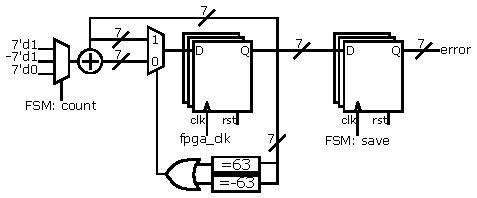
\includegraphics[width=0.8\textwidth]{../updown}
	\caption[\ac{RTL} diagram of up-down counter]{\ac{RTL} diagram of up-down counter.}
	\label{fig:updown_ctr}
\end{figure}

A major pitfall was encountered in this design of phase detector, which lead in some conditions to a form of mode-locking, in which each oscillator would lock $180\si{\degree}$ phase shifted from the oscillators used as a reference. This was later discovered to be as a result of the measurement interval termination conditions in the \ac{FSM}, which in addition to those described in Figure \ref{fig:state_trans_reprint}, would terminate the interval if a falling edge was observed on the signal that originally triggered the measurement. Figure \ref{fig:uncertainty} will be used to describe the exact circumstances of the error.
\begin{figure}[h]
	\centering
	
\includegraphics[width=0.6\textwidth]{../uncertain}
	\caption[Circumstances of mode locking behaviour]{Circumstances of mode locking behaviour.}
	\label{fig:uncertainty}
\end{figure}

The situation would occur when the measurement interval began with a large phase difference between the generated and reference signals and a simultaneous difference in frequency. Without a frequency difference the measurement beginning at ``interval start'' would terminate at location ``a'', measuring a large lag, with the following measurement interval starting at location ``d''. However in the presence of a frequency differential, the rising edge on the generated signal may occur only at location ``c'', and with the falling edge termination condition causing the interval to terminate before this edge was detected, at point ``b''. This lead to a slightly lower magnitude phase lag detected, however this is a minor flaw, and not the cause of the mode locking. As the rising edge at point ``c'' occurs after the interval has terminated, it is treated as a fresh measurement interval, terminating at ``d''. As in this interval, the generated signal has seen the first rising edge, a large lead will be recorded. As each correction is made with a delay of one cycle, in order to avoid timing violations in the feedback path, there is potential for oscillation between lead and lag detection to occur depending on the initial conditions. This low probability behaviour was observed by chance, due to coding error, while using a frequency divider in the feedback path as this ensured the lead and lag measurements were of identical magnitude. 

\subsubsection{Simulations}
%TODO simulations
As this was the first \ac{ADPLL} design implemented, various Vivado test benches were used to verify the behaviour of each module. Simulations with this design were made more efficient due to deterministic timing in all modules, and absence of any inverter based components which required the use of post-implementation simulations in order to avoid zero delay oscillations. Deterministic timing means \ac{ADPLL} 1 offers an additional, and significant, advantage over other designs as it can be entirely simulated in Vivado with accurate timings. This ability was vital initially, as it revealed the presence of edge situations that had not been accounted for, and through exporting the waveforms to a log file and analysis performed using Matlab comparison made to the measured system behaviour.

\begin{figure}[h]
	\centering
	\subfloat[Vivado simulation.]{{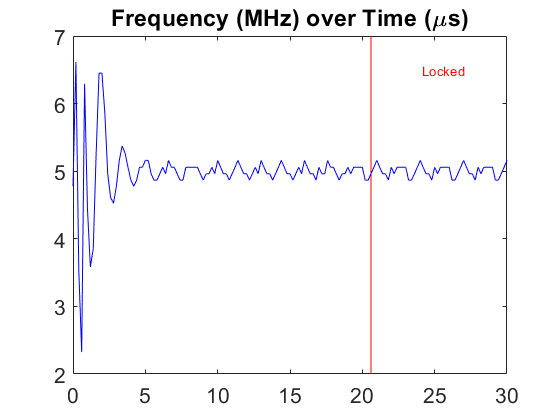
\includegraphics[width=0.45\textwidth]{../sim_locking} }}\\
	\subfloat[Hardware measurement.]{{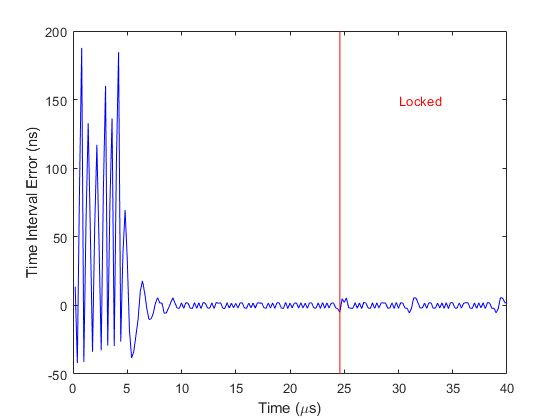
\includegraphics[width=0.45\textwidth]{../impl_locking} }}%
	\caption[\ac{ADPLL} 1 Vivado locking simulations]{\ac{ADPLL} 1 Vivado locking simulations.}
	\label{fig:sim_locking}
\end{figure}
In Figure \ref{fig:sim_locking} (a), the startup behaviour of the system can be observed. This simulation was performed with a reference at exactly $5~\si{\mega\hertz}$ and an initial deviation of $252~\si{\kilo\hertz}$, and the plot shows the inverse of the \ac{DCO} period against the time since the oscillator was enabled. After some initial oscillation the period settles around that of the reference. Once locked, cycle-to-cycle jitter was calculated to be $3.491~\si{\nano\second}$ using the standard deviation of the periods, with a worst case cycle-to-cycle change of $9.299~\si{\nano\second}$. Lock was visually determined to have occurred after $20.91~\si{\micro\second}$, after which the oscillator frequency began to change in a repetitive pattern. later the same test carried in hardware with identical initial conditions, the results of which are shown in Figure \ref{fig:sim_locking} (b). This plot is derived from data captured using an Agilent MSO7054A, using a setup that will be further explained in Section \ref{section:measurement_setup}. Despite lacking a non ideal reference, less violent initial oscillation, and a lesser until lock could be visually determined, the simulation provided a good insight into the system's behaviour once implemented on an \ac{FPGA}.



\subsubsection{\acs{ADPLL} 1 Design Summary}
The listed components were brought together in \textsc{NetworkADPLL.v}, attached in Appendix \ref{adx:code} Listing \ref{lst:network_adpll}. Important to note is that each \ac{ADPLL} only contains two \acl{PD}s despite during network operation the need for phase comparisons to be made with up to four neighbours. The two ``missing'' \ac{PD}s are in fact synthesised as part of the other \ac{ADPLL}s, with which the comparison would be made. This allows for a 50\% reduction in the number of \ac{PD}s required, while also ensuring identical error is received by both \ac{ADPLL}s. Each \ac{ADPLL} performs comparison with the \ac{DCO} ``above'' and ``left'' of them in the Cartesian grid, and a port in the module outputs the results for use by the other \ac{ADPLL}s involved. %TODO juvenile wording
Table \ref{table:adpll1} contains a brief overview of the bit widths, tuning ranges and other configuration information for this \ac{ADPLL}.
\begin{table}[!h]
	\begin{center}
		\begin{tabular}{|l|r|r|r|}
			\multicolumn{4}{c}{\ac{DCO} Tuning Range} \T\\
			\hline
			\multicolumn{1}{|c|}{-} & \multicolumn{1}{c|}{Minimum} & \multicolumn{1}{c|}{Step} & \multicolumn{1}{c|}{Maximum} \T\\
			\hline
			Frequency & $1.008~\si{\mega\hertz}$ & \multicolumn{1}{r|}{$62.988~\si{\kilo\hertz}$} & $8.944~\si{\mega\hertz}$ \T\\
			\hline
			Period & $992.0~\si{\nano\second}$ & \multicolumn{1}{r|}{$2.5~\si{\nano\second}$ (at $5~\si{\mega\hertz}$)} & $111.8~\si{\nano\second}$ \T\\
			\hline
		\end{tabular}
		\begin{tabular}{|l|r|l|r|}
			\multicolumn{4}{c}{Configuration as Implemented} \T\\
			\hline
			\ac{DCO} Counter Width & 12 bits & \ac{DCO} Control Width (max) & 12 bits \T\\
			\hline
			\ac{DCO} Bias Point & 79 & Runtime Gains & Enabled \T\\
			\hline
			Phase Detector Error Width & 7 & Error Sum Weight Width & 4 \T\\
			\hline
			\acs{kp} & $2^{-5}\times[0,15]\cap\mathbb{Z}$ & \acs{ki} & $2^{-8}\times[0,15]\cap\mathbb{Z}$ \T\\
			\hline
			Detection Resolution & $3.875~\si{\nano\second}$ & Detection Phase Resolution & $6.975\si{\degree}$ (at $5~\si{\mega\hertz}$)\\
			\hline
		\end{tabular}
	\end{center}
\caption[ADPLL Design 1 Summary]{ADPLL Design 1 Summary.}
\label{table:adpll1}
\end{table}

\subsection{\acs{ADPLL} Design 2}
The second \ac{ADPLL} design implemented during the course of this project was somewhat of a stepping stone between fully synchronous and asynchronous to the \ac{FPGA} clock. The clocked phase detector is reused from above, albeit with an altered error width, while the \ac{DCO} is replaced by a \acl{RO}. While the phase detector was known to work due to testing in \ac{ADPLL} 1, the \ac{DCO} could not be simulated using accurate timings so all testing had to be done in hardware. This presented a challenge, as depending on the implementation, the characteristics of the \ac{DCO} could change, most importantly the centre frequency. The module implementing this \ac{ADPLL} can be found in \textsc{NetworkRingADPLL.v}, attached in Appendix \ref{adx:code} Listing \ref{lst:network_ring_adpll}.

\subsubsection{\acl{DCO}}
\ac{ADPLL} 2 exchanges the \ac{FPGA} clocked oscillator for \ac{RO}, with the aim of obtaining performance more akin to that of an \ac{ASIC} based mixed-signal implementation, due to the variation in period steps both between oscillators and within the same oscillator due to the oscillator layout. Also advantageous is the improvement in period resolution obtained using this design, when compared to that of the \ac{FPGA} clocked design. Taking the formula given in Chapter \ref{chap:3} and the inverter propagation time used by Vivado in post synthesis/implementation simulations of $315~\si{\pico\second}$, the period step can be computed:
\begin{align}
t_{step} &= \text{inverters per step}\times\text{inversions per period}\times\text{propagation delay} \\
t_{step} &= \text{inverters per step}\times\text{inversions per period}\times\tau_{inv} \\
t_{step} &= 2\times 2\times 315~\si{\pico\second} = 1.26~\si{\nano\second}
\end{align}
Using the propagation delay, $\tau_{inv}$, the number of inverters required to produce the signal of period $200~\si{\nano\second}$ can easily be computed:
\begin{equation}
\text{num\_inverters} = \left \lfloor{ T_{osc~@~5~\si{\mega\hertz}}\times \frac{1}{2\times\tau_{inv}}}\right \rceil = \left \lfloor{ \frac{200~\si{\nano\second}}{0.63~\si{\nano\second}}}\right \rceil = 317
\end{equation}

\begin{figure}[h]
	\centering
	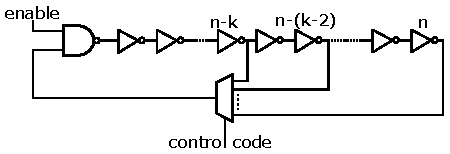
\includegraphics[width=0.8\textwidth]{../ro_new}
	\caption[\acl{RO} RTL diagram]{\acl{RO} RTL diagram.}
	\label{fig:ro_impl}
\end{figure}
Figure \ref{fig:ro_impl} contains an \ac{RTL} diagram of the \ac{RO} as implemented. The inverter chain is specified with a maximum length of $n$ and a maximum number of removable inverters of $k$. In order to preserve the unstable circuit, by maintaining an odd number of inverters, only multiples of two inverters may be removed at a time. The already introduced \ac{DCO} and \ac{PFD} designs all followed the same convention regarding phase error and the corresponding impact on the control code: In the \ac{PFD}, if the generated signal was lagging the reference, meaning it should ``go faster'' in order to ``catch up'', the error given a positive sign. Similarly in the \ac{FPGA} clocked \ac{DCO}, a positive change in the magnitude of the control code resulted in a higher frequency. In the interests of consistency and extensibility the same behaviour was implemented for this \ac{DCO} also, with the number of inverters in the chain given as:
\begin{equation}
\text{num inverters} = n - 2\times CC,~CC<\frac{k}{2}
\end{equation}
Where $CC$ is the unsigned integer control code input. $k$ is determined by the bit width of the control code which, as in the case of the clocked \ac{DCO}, is also an unsigned number. An inverter chain will oscillate freely and cannot be disabled. To this end the first inverter in the chain was replaced by a \acs{NAND} gate to grant control over its operation.

The bias point functions differently in this oscillator, as unlike the \ac{FPGA} clocked design it is not required to set the centre of the tuning range, as in the \ac{RO} this lies at $n-\frac{k}{2}$. Instead the bias point servers as a conversion between the signed \ac{LF} output, which is in two's complement form, and the unsigned requirement of the control code. This is achieved by adding on the midpoint of the unsigned range and storing the result in an unsigned value. Using the case where the width of the control code is three: The range of the signed three bit integer is from $-4$ (100) to $3$ (011) which when directly converted to unsigned values become $4$ and $3$, thus destroying the relationship between lead and lag. Worse still the signed value of $-1$ (111) becomes $7$. Adding on the mid range value solves this problem, with a signed value of $-4$ now mapping to $0$ and $3$ to $7$. Comparing this behaviour to response of the \ac{RO} to the control code, it can be trivially seen that the minimum possible period will still correspond to the largest control code prior to conversion and vice versa for the maximum period.

A control code width of 5 bits was chosen, as with two inverters removed per control code, the tunable range would consist of $20\%$ of the total inverter count. To achieve this range with a centre of $317$ inverters, the maximum number of inverters in the chain was required to be $317+2\times 2^{5-1} = 349$, dropped to a minimum at $285$. The corresponding minimum and maximum frequencies then are:
\begin{align}
f_{osc} &= \frac{1}{T_{osc}} = \frac{1}{(n-2CC)\times 2\times\tau_{inv}} = \frac{1}{(n-2CC)\times 2\times 315~\si{\pico\second}} \\
f_{min} &= \frac{1}{T_{max}} = \frac{1}{349\times 2\times 315~\si{\pico\second}} = 4.548~\si{\mega\hertz} \\
f_{max} &= \frac{1}{T_{min}} = \frac{1}{285\times 2\times 315~\si{\pico\second}} = 5.569~\si{\mega\hertz}
\end{align}

The first pitfall with this type of \ac{DCO} comes in the \ac{HDL} stage, with the \ac{EDA} likely to optimise away what it sees as a long chain of inverters carrying out no function. This can be avoided by adding an \texttt{attribute} as a prefix to the instantiation of a logic element or net that should not be ``optimised'' away. It is important to choose the correct directive, otherwise the compiler may not behave as expected. In the case of Vivado, it is important not to confuse the \texttt{KEEP} or \texttt{KEEP\_HIERARCHY} commands with that of \texttt{DONT\_TOUCH}, with former commands only ensuring that the logic elements will be maintained in synthesis, but not in any subsequent stages \cite{synth_ug}.

As mentioned in previous chapters, the absence of direct control over layout can lead to significant variation of the propagation time though inverters. This may occur in three ways: Firstly, the layout of individual \ac{RO}s may be significantly different, thus resulting in poor overlap of tuning regions. Anecdotally, while implementing a 3x3 network, 7 of the 9 oscillators had centre frequencies within a $100~\si{\kilo\hertz}$ span but two lay more than $500~\si{\kilo\hertz}$ away in opposite directions which prevented the network from locking. Secondly, within an \ac{RO} the propagation delay between each inverter may vary, which results in a variable frequency step, possibly changing the locking range. These two effects represent an extreme version of the variation due to process or manufacturing seen on \ac{ASIC}s. The final variation is possibly the most frustrating, and occurs when between implementations the \ac{EDA}, Vivado in the case of this project, changes the layout of the \ac{RO}. This may occur as a result of a direct change, or as a result of seemingly innocuous changes to unrelated modules. While the final problem can be avoided, once the performance of the \ac{RO} is satisfactory, by locking down module, the remaining two problems can only be mitigated somewhat.

This is achieved by assigning specific areas of the chip in which that module must lie, although these must be of a size approximately $40\%$ larger than the minimum space required in order to avoid having the router create a complex, delay intensive layout to fit the \ac{RO}. To achieve greater consistency, the implementation directive can be modified such that the router will attempt to use the minimum area that does not require complex routing. \texttt{congestion\_spreadlogic\_low} was used for this purpose in this project, although other options may obtain similar results. The other options available in Vivado can be viewed in the \textit{Vivado Design Suite User Guide - Implementation} \cite{impl_ug}.

With the hardware description of the \ac{RO} completed, testing of an instance of the \ac{RO} with a constant control code of zero was attempted, and it was discovered that the estimation of the centre frequency based on the propagation delay was off by $100$s of $\si{\kilo\hertz}$. The addition of 100 inverters was required to restore a centre of $5~\si{\mega\hertz}$. After the \ac{RO} was integrated into \ac{ADPLL} 2 the centre frequency was discovered to have changed once more. The minor variation caused by the now variable control code had changed the average propagation delay through the inverters once more, now requiring 373 inverters for $5~\si{\mega\hertz}$.
%TODO possibily problematic in the last two paragraphs

When, later in the project, additional \ac{RO}s were implemented to form networks, 373 inverters proved a suitable starting point which consistently delivered \ac{DCO}s with a centre frequency within $200~\si{\kilo\hertz}$ of $5~\si{\mega\hertz}$. For the purposes of describing a typical tuning range, the average propagation delay of an \ac{RO} consisting of 373 inverters with a centre frequency of $5.06~\si{\mega\hertz}$ will be used. To avoid the aforementioned issues with constant control codes, the fixed code was achieved by implementing an \ac{ADPLL} and setting the \ac{PI} filter gains to zero at runtime before performing a reset.

Using this updated maximum number of inverters the frequency range can be recalculated. Firstly, the new minimum and maximum numbers of inverters are $309$ and $373$ respectively, with a mid point at $341$. The inverter delay and period step are then recomputed based on the centre frequency of $5~\si{\mega\hertz}$ as:
\begin{align}%TODO 2 x 2 x midpoint justification - in prev. chapter?
t_{step} &= \frac{T_{osc}}{0.5\times(n-\frac{k}{2})} = \frac{200\si{\nano\second}}{0.5\times 341} = 1.176~\si{\nano\second} \\
\tau_{inv} &= \frac{t_{step}}{2\times\text{inverters per step}} = \frac{t_{step}}{2\times2} = \frac{1.176~\si{\nano\second}}{4} = 293~\si{\pico\second}
\end{align}
The frequency range is then:
\begin{align} %TODO inconsisentl calculation approach with previous version
f_{osc} &= \frac{1}{T_{osc}} = \frac{1}{(n-2CC)\times 2\times\tau_{inv}} \\
f_{min} &= \frac{1}{T_{max}} = \frac{1}{(373-0)\times 2\times 293~\si{\pico\second}} = 4.571~\si{\mega\hertz} \\
f_{max} &= \frac{1}{T_{min}} = \frac{1}{(373-2\times32)\times 2\times 293~\si{\pico\second}} = 5.518~\si{\mega\hertz}
\end{align}

The module implementing the \ac{RO} can be found in \textsc{RingOsc.v}, attached in Appendix \ref{adx:code} Listing \ref{lst:ring_osc}.

\subsubsection{Phase Detector}
The \ac{PFD} used in this oscillator is, apart from the bit width of the counter, identical to that used in the previous design. The reduction in counter width will have no impact of performance of the \ac{ADPLL} once a lock has been acquired, however, the capture speed will be reduced for large phase differences due to the counter reaching saturation point significantly sooner. 5 bits corresponds to a counter range of $[-15,15]\cap\mathbb{Z}$, which will saturate at a time delay of $15\times3.875\si{\nano\second} = 58.125~\si{\nano\second}$, a phase lead or lag of $\frac{}{}\times360\si{\degree} = 104.4\si{\degree}$ at $5~\si{\mega\hertz}$. This is an adequate range, as saturation will occur well outside of the normal operating range. This reduction is most noticeable when a divider is active in the feedback path, however during locked operation a phase shift of $58.125~\si{\nano\second}$ will not occur, so this impact is only felt during acquisition.

\subsubsection{\acs{ADPLL} 2 Design Summary}
As previously mentioned, \ac{ADPLL} 2 represents a midway point between \ac{FPGA} clocked designs and those which are asynchronous. As the source of the asynchronicity is the inverter chain \ac{DCO}, a more realistic jitter would be expected from this design, with there being a significant distribution of period steps. Among other aspects, this will have a noticeable impact in steady state conditions, where the degree of fractional synthesis required will vary from oscillator to oscillator depending on the closest distance from the reference period to a period obtainable by the individual oscillator. This is a source of jitter that was not present in the clocked \ac{DCO} used in \ac{ADPLL} 1, as all period steps were equal. Once again the \ac{DCO} tuning ranges and configuration details for future measurements are listed below, in Table \ref{table:adpll2}.

\begin{table}[!h]%TODO redo numbers!
	\begin{center}
		\begin{tabular}{|l|r|r|r|}
			\multicolumn{4}{c}{\ac{DCO} Tuning Range} \T\\
			\hline
			\multicolumn{1}{|c|}{-} & \multicolumn{1}{c|}{Minimum} & \multicolumn{1}{c|}{Step} & \multicolumn{1}{c|}{Maximum} \T\\
			\hline
			Frequency & $4.571~\si{\mega\hertz}$ & $29.180~\si{\kilo\hertz}$ (at $5~\si{\mega\hertz}$) & $5.518~\si{\mega\hertz}$ \T\\
			\hline
			Period & $218.2~\si{\nano\second}$ & $1.176~\si{\nano\second}$ & $181.1~\si{\nano\second}$ \T\\
			\hline
		\end{tabular}
		\begin{tabular}{|l|r|l|r|}
			\multicolumn{4}{c}{Configuration as Implemented} \T\\
			\hline
			\ac{RO} num. of inverters (max) & 373 & \ac{RO} Control Width & 5 bits \T\\
			\hline
			\ac{RO} Bias Point & 16 & Runtime Gains & Enabled \T\\
			\hline
			Phase Detector Error Width & 5 & Error Sum Weight Width & 4 \T\\
			\hline
			\acs{kp} & $2^{-7}\times[0,15]\cap\mathbb{Z}$ & \acs{ki} & $2^{-9}\times[0,15]\cap\mathbb{Z}$ \T\\
			\hline
			Detection Resolution & $3.875~\si{\nano\second}$ & Detection Phase Resolution & $6.975\si{\degree}$ (at $5~\si{\mega\hertz}$)\\
			\hline
		\end{tabular}
	\end{center}
	\caption[\ac{ADPLL} Design 2 Summary]{\ac{ADPLL} Design 2 Summary.}
	\label{table:adpll2}
\end{table}


\subsection{\acs{ADPLL} Design 3}
\acs{ADPLL} Design 3 has no dependence on the clock provided by the \ac{FPGA}'s clock management utility, as both the \ac{RO} and the \ac{TDC} are designed using inverters, while a Bang-Bang detector replaces the \ac{FPGA} clock reliant \ac{FSM} of the two previous designs. This introduces a second source of implementation based variation between \ac{ADPLL}s, however, this has significantly lesser impact on the frequency range of the oscillator and no impact on the centre frequencies. The lack of an \ac{FPGA} clocked element results means this design will have the closest behaviour to that of an \ac{ASIC} based \ac{ADPLL} implementation, although as the level of variation due to implementation is much larger on an \ac{FPGA}, the impact of non-idealities will be exaggerated.
%same interface
In order to allow quick exchange of \ac{PD}s or other modules, the module in which this \ac{ADPLL} is implemented is still retains the \ac{FPGA} clock as an input. In fact, this module shares its implementation with that of \ac{ADPLL} 2, as while the \ac{PD} designs are drastically different, the interface is identical. The module implementing this \ac{ADPLL} can be found in \textsc{NetworkRingADPLL.v}, attached in Appendix \ref{adx:code} Listing \ref{lst:network_ring_adpll}.

\subsubsection{\acl{DCO}}
The \ac{DCO} used in \ac{ADPLL} 3 is identical in form to that used in \ac{ADPLL} 2, so the tuning range, period step and all effects of implementation variations carry over to this \ac{ADPLL}. The decision to leave the \ac{RO} unmodified is an easy one, as the intended centre frequency is the same and changing the control code width would remove the ability to fix the cells of each \ac{RO}. Fixing the cells is beneficial as it will maintain the oscillator layout between implementation ``runs'', and thus allow for a better comparison between designs 1 \& 2.

\subsubsection{Phase Detector}
Instead of an \ac{FPGA} clocked phase detector, \ac{ADPLL} 3 uses the modified Bang-Bang detector and \ac{TDL} approach to phase comparison seen in Section \ref{section:signum}. Sign detection is implemented exactly as described in that section, with the double \ac{SR} latch approach used to determine the sign of the phase error. A flip-flop is inserted after the second \ac{SR} latch, clocked on the signal \texttt{done}, which holds the output value and ensures that the sign changes at the same time as the magnitude. The previous discussion of this phase detector proposed no implementation of the edge detectors, which are easily implemented using flip-flops clocked on the signal of interest, with a constant $1$ on the $D$ input. In this form the edge detector is single use only, as subsequent edges will not cause any change in the flip-flop output. This is important as it ensures the measurement interval will only terminate when a rising edge is seen on the signal that did not start the measurement interval, thus avoiding the mode locking seen in the original implementation of the \ac{FPGA} clocked \ac{PD}. Once the measurement interval has completed, the \texttt{done} signal is used to reset the edge detectors asynchronously. It is possible that an edge may occur within the time taken to reset the counters, and thus the detector incorrectly gauge the start of a measurement interval, however this can only occur in exceptional circumstances in the acquisition period. Therefore it is possible to ignore this scenario, as the only impact will be an increased time taken to acquire a lock.
\begin{figure}[h]
	\centering
	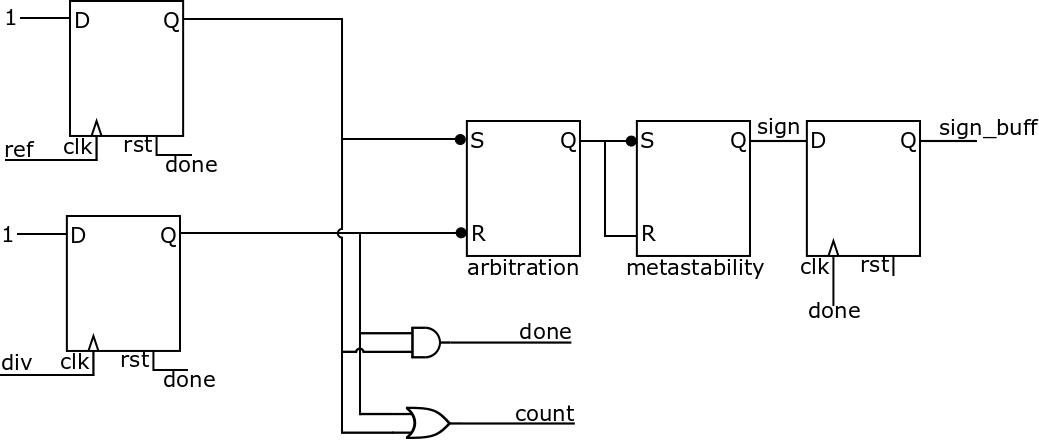
\includegraphics[width=0.8\textwidth]{../new_pdet1}
	\caption[Modified Bang-Bang sign detector RTL diagrams]{Modified Bang-Bang sign detector RTL diagrams.}
	\label{fig:signdet_impl}
\end{figure}

A two signal interface controls the \ac{TDC}, a \texttt{count} that enables the \ac{TDC} and a \texttt{done} signal that signals the termination of the interval. A single logic gate is required to generate each signal, as ORing the two edge detector outputs will produce logic $1$ when the interval has begun while ANDing these signals will indicate the end of the interval when both edges have occurred. The \texttt{done} signal is also used to clock the flip-flop acting as a buffer for the sign. The exact implementation of the sign detection circuit can be seen in Figure \ref{fig:signdet_impl}.

As previously mentioned, the time-to-digital conversion is carried out by a tapped delay line. As with the \ac{RO}, inverters will be used to provide the delay between each tap, and thus the resolution of the \ac{TDL} and the length of each individual delay is based on the layout chosen by the router in Vivado. Due to this, the exact resolution of the phase detector is unknown, although the delay through inverters used in Vivado simulations and the average delay computed based on \ac{RO} centre frequencies can be used to estimate that of the phase detectors. Based these figures for the the propagation delay due to an inverter, $\tau_{inv}$ can be estimated to be in the region of $300~\si{\pico\second}$. As each tap consists of an inverter pair, the delay through the tap, $\tau_{tap} \approx 600~\si{\pico\second}$. Characterisation of the \ac{TDL}, and thus measurement of the delays in each \ac{TDL}, is technically possible, however, this is an time consuming process as many \ac{TDL}s would need to be characterised in order to accurately compute the average delay. 

%TODO eugene
The delay line itself is shown in Figure \ref{fig:tdl_impl}, with each tap implemented by a pair of flip-flops and three inverters. For an $N$ bit width phase error detection, $2^{N-1}-1$ taps are required. In the case of this \ac{ADPLL}, a 5 bit two's complement error signal is required, thus the range of the signal is $[-16,15]\cap\mathbb{Z}$. If the range is made symmetrical, 15 taps are required to fill a signal of this size. From the diagram it can be seen that unless edges are detected on each signal at exactly the same instant, it is almost impossible to measure a zero phase difference between reference and generated signals. This is an intentional decision, \cite{idkwhattocite}.
\begin{figure}[h]
	\centering
	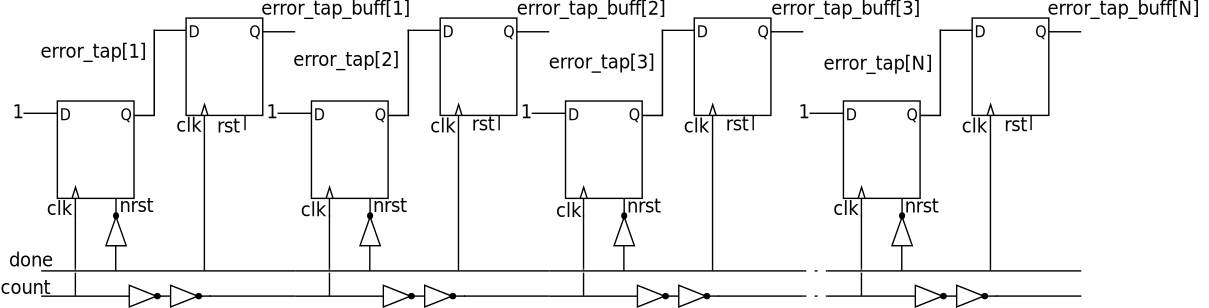
\includegraphics[width=1.0\textwidth]{../new_pdet2}
	\caption[Inverter based \ac{TDL} RTL diagrams]{Inverter based \ac{TDL} RTL diagrams.}
	\label{fig:tdl_impl}
\end{figure}
The operation of the \ac{TDL} is as follows: A delayed version of the \texttt{count} signal acts as the clock for flip-flops forming each tap, which are rising edge activated. These flip-flops have a constant ``1'' at their $D$ inputs, so as the signal propagates through the delay line, each flip-flop with propagate a logic ``1'' to their corresponding \texttt{error\_tap[i]} signal. When the measurement interval has completed, the \texttt{count} signal clocks the 15 bit wide \texttt{error\_tap} signal into \texttt{error\_tap\_buff} which act as the output buffers of the \ac{PD}, holding the phase error constant between measurement intervals. As with the flip-flops performing edge detection, the flip-flops comprising the taps can only be used once before requiring a reset, which is again carried out using the \texttt{done} signal. As flip-flops have a hold time, the duration after the clock edge in which the signal applied at the $D$ input must not change to ensure valid data, an inverter is used to delay the reset to avoid this issue.

The output of the \ac{TDL} itself is not a binary signal, but rather the thermometer coded representation of the number of taps activated in the measurement interval. In order to convert to binary, the easiest solution is a switch statement, with an assignment performed based on the temperature code. However all \ac{ADPLL} blocks have been designed to be extensible, requiring the lookup to be generated at compile time. This is somewhat difficult to implement, and a simpler solution exists for this problem. In a \texttt{generate} statement, a variable size loop is used to count the number of nonzero bits as it would be done in C. At compile time this loop is converted into lookup tables, similarly to the switch statement.

The now unsigned binary representation of the error magnitude can be combined then with the sign bit to form a two's complement error signal. The file \textsc{PhaseDetectorDL.v} in Appendix \ref{adx:code} Listing \ref{lst:phase_detector_dl} contains the Verilog implementation of this module. \texttt{DONT\_TOUCH} compiler directives were used here in a number of places to ensure that the inverters and other elements that are key for timing are not removed in the synthesis process, as similarly to \ac{RO}, Vivado sees these as unneeded elements serving no purpose.

\subsubsection{\acs{ADPLL} 3 Design Summary}
Table \ref{table:adpll3}.

\begin{table}[!h]%TODO numbers!
	\begin{center}
		\begin{tabular}{|l|r|r|r|}
			\multicolumn{4}{c}{\ac{DCO} Tuning Range} \T\\
			\hline
			\multicolumn{1}{|c|}{-} & \multicolumn{1}{c|}{Minimum} & \multicolumn{1}{c|}{Step} & \multicolumn{1}{c|}{Maximum} \T\\
			\hline
			Frequency & $4.571~\si{\mega\hertz}$ & $29.180~\si{\kilo\hertz}$ (at $5~\si{\mega\hertz}$) & $5.518~\si{\mega\hertz}$ \T\\
			\hline
			Period & $218.2~\si{\nano\second}$ & $1.176~\si{\nano\second}$ & $181.1~\si{\nano\second}$ \T\\
			\hline
		\end{tabular}
		\begin{tabular}{|l|r|l|r|}
			\multicolumn{4}{c}{Configuration as Implemented} \T\\
			\hline
			\ac{RO} num. of inverters (max) & 373 & \ac{RO} Control Width & 5 bits \T\\
			\hline
			\ac{RO} Bias Point & 16 & Runtime Gains & Enabled \T\\
			\hline
			Phase Detector Error Width & 5 & Error Sum Weight Width & 4 \T\\
			\hline
			\acs{kp} & $2^{-7}\times[0,15]\cap\mathbb{Z}$ & \acs{ki} & $2^{-9}\times[0,15]\cap\mathbb{Z}$ \T\\
			\hline
			Detection Resolution & $3.875~\si{\nano\second}$ & Detection Phase Resolution & $6.975\si{\degree}$ (at $5~\si{\mega\hertz}$)\\
			\hline
		\end{tabular}
	\end{center}
	\caption[\ac{ADPLL} Design 3 Summary]{\ac{ADPLL} Design 3 Summary.}
	\label{table:adpll3}
\end{table}


\section{Measurement Setup}\label{section:measurement_setup}
For the following sections in which the performance of either individual \ac{ADPLL}s or \ac{ADPLL} networks the same measurement setup was used. The \ac{FPGA} used was a Xilinx Artix-7 \acl{Nexys} on a Digilent \acs{Nexys} board. The \acl{Nexys} features 15850 logic slices, each with 4 lookup tables and 8 flip-flops. There are six clock management tiles, 240 dedicated digital signal processing slices and an analog-to-digital converter. The maximum operating frequency is $464~\si{\mega\hertz}$ and 210 input/output ports are available for use. Further information can be found in the datasheet \cite{a7_datasheet}. The \acs{Nexys} is an evaluation/development board for the aforementioned \ac{FPGA}, however directed at the education sector. It contains useful peripherals such as 16 switches, 8 7-segment displays and 4 user addressable \ac{PMOD} headers and can be used with the free of charge ``Webpack'' version of Vivado \cite{n4_datasheet}.
\begin{figure}[h]
	\centering
	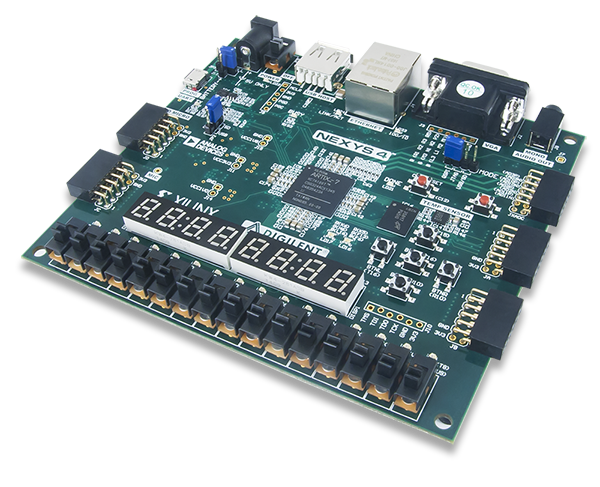
\includegraphics[width=0.6\textwidth]{../n4}
	\caption[\acs{Nexys} development board]{\acs{Nexys} development board.}
	\label{fig:n4}
\end{figure}

Measurements were performed using an Agilent MSO7054A, a four channel, $4~\si[per-mode=symbol]{\giga\sample\per\second}$ oscilloscope. Signals were extracted over the regular \ac{PMOD} headers as the board does not provide outputs better suited to the measurement of signals that are available to the user, such as SMA or BNC connectors, and the \ac{PMOD} header for the analog-to-digital converter, which has lower impedance traces, is not available for the designer to re-configure. Data was acquired with the oscilloscope in quad channel mode at a sampling rate of $2\si{\giga\sample\per\second}$. One of the four channels was consumed by the external reference, leaving three free for signal measurements, in most cases the generated output of three \ac{ADPLL}s were connected. $200\si{\micro\second}$ long captures were saved to an Agilent specified binary format which could be opened in Matlab for analysis.
%TODO diagram or picture of some sort

\section{\acs{ADPLL} Characterisation}
%TODO why each PLL

\section{Minor Variations}\label{section:minor_variations}
%TODO osc size

\section{\acs{ADPLL} Network Implementation}
\subsection{2x2 Network}
\subsection{3x3 Network}


\setcounter{chapter}{4}

\chapter{Testing and Analysis}\label{chap:5}

\section{Chapter Overview}
This chapter contains details of the measurements carried out on networks of various sizes in addition to investigation into the impact of a number of decisions made in the design process. Explanations will be given, or analysis made, of the results, which will be either in the form of plots or tables, depending on which allows for more concise presentation of the data. Both 2x2 and 3x3 network performance analysis was performed with no input delay to the \ac{LF}, which Section \ref{subsection:lf_delay} will show to have had a significant performance impact. Unless otherwise stated, all tests were carried out at a centre frequency of $5~\si{\mega\hertz}$.

\section{2x2 Network Performance Comparison}
In order to investigate the impact of the \ac{ADPLL} network on performance, and conversely the impact of each individual \ac{ADPLL} design on the network, switches were used to alter the configuration of the network without requiring re-implementation. A number of captures were made at each setting. The three configurations were: each \ac{ADPLL} individually locked to the reference, the network in uni-directional mode and in bi-directional mode. In order to obtain a good comparison, the \ac{LF} gains were not changed between measurements. For \ac{ADPLL} 1 the gains were: $k_p = \frac{1}{32}$ \& $k_i = \frac{1}{256}$. For \ac{ADPLL} 2 and 3 they were: $k_p = \frac{1}{16}$ \& $k_i = \frac{1}{64}$. \ac{ADPLL} requires a smaller gain due to the greater frequency sensitivity.

\begin{table}[!ht]
    \begin{center}
        \begin{footnotesize}
            \setlength{\tabcolsep}{.9\tabcolsep}
            \begin{tabular}{ll|r|r|r|r|r|r|r|r|r|}           
                \cline{3-11}
                && \multicolumn{3}{c|}{Jitter Standard Deviation (ns)} & \multicolumn{3}{c|}{Max. Time Interval Error (ns)} & \multicolumn{3}{c|}{Skew (ns)} \T\\
                \cline{3-11} 
                &&PLL 11&PLL 12&PLL 22    &PLL 11&PLL 12&PLL 22    &PLL 11&PLL 12&PLL 22\T\\
                \hline
                \multicolumn{2}{|l|}{\ac{ADPLL} Design 1}&-&-&-&-&-&-&-&-&-\T\\
                \multicolumn{2}{|r|}{Free PLLs} &1.6051  &1.6146  &1.6251     &1.6985 &1.5833 &1.2712    &0.2700 &0.5817 &0.2491 \T\\
                \multicolumn{2}{|r|}{Uni-dir.}  &1.7693  &1.8463  &1.8862     &7.3060 &7.2565 &10.151    &2.2791 &1.2822 &1.6299 \T\\
                \multicolumn{2}{|r|}{Bi-dir.}   &1.9964  &1.9146  &1.9572     &15.089 &18.283 &19.673    &9.2449 &11.612 &12.052 \T\\
                \hline
                \multicolumn{2}{|l|}{\ac{ADPLL} Design 2}&-&-&-&-&-&-&-&-&-\T\\
                \multicolumn{2}{|r|}{Free PLLs} &0.66275 &0.62108 &0.63211    &5.7432 &5.4399 &5.2317    &0.00768 &-0.1681 &0.5383  \T\\
                \multicolumn{2}{|r|}{Uni-dir.}  &0.65990 &0.63995 &0.67278    &5.6926 &6.9422 &8.9609    &0.00663 &-0.3453 &0.76741 \T\\
                \multicolumn{2}{|r|}{Bi-dir.}   &0.66308 &0.66233 &0.67583    &12.222 &16.719 &19.176    &5.0799  & 7.2752 &8.7174  \T\\
                \hline
                \multicolumn{2}{|l|}{\ac{ADPLL} Design 3}&-&-&-&-&-&-&-&-&-\T\\
                \multicolumn{2}{|r|}{Free PLLs} &0.66757 &0.84477 &0.71308    &5.9142 &6.1353 &5.3939    &-0.36997 &-0.20981 &-1.3344  \T\\
                \multicolumn{2}{|r|}{Uni-dir.}  &0.66934 &0.83894 &0.71271    &5.8779 &7.1746 &6.8914    &-0.36645 &-0.05647 &-0.36178 \T\\
                \multicolumn{2}{|r|}{Bi-dir.}   &0.68372 &0.83193 &0.68570    &7.5705 &9.6292 &9.7715    & 0.68901 & 1.58720 & 1.5553  \T\\
                \hline
                \B                
            \end{tabular}
        \end{footnotesize}
        \caption{2x2 Network Performance Comparison.}
        \label{table:2x2perf}
    \end{center}
    \vspace{-0.5cm}
\end{table}
There are two main trends worth highlighting here, the first of these being as the feedback network becomes more complicated a large degree of skew is introduced, with the magnitude becoming larger in the \acp{ADPLL} further from the reference. This would appear to be attributable to a combination of the time taken for a change in the reference to propagate to the \ac{ADPLL} node in question, and the fineness of period and detection resolutions. This second observation follows from the significant reduction in the skew growth in Designs 2 \& 3 which have finer resolutions. 

The other trend, is the variation in \ac{C2C} jitter across the \ac{ADPLL} designs, with coarseness of the \ac{FPGA} clocked \ac{DCO} becoming somewhat obvious. As free \aclp{PLL} (\acsp{PLL}), the clocked \ac{DCO} has almost identical \ac{C2C} jitter and maximum \ac{TIE}, implying that only two period steps are used the majority of the time. As, at $3.875~\si{\nano\second}$, these steps are somewhat further apart than that of the \ac{RO} (an implementation dependant value in the region of $1.1765~\si{\nano\second}$), a much greater jitter is observed. This would confirm the belief that the \ac{FPGA} clocked designs are better suited to operational frequencies where the generated clock period is multiple orders of magnitude longer than the \ac{FPGA} clock period. In this design, the ratio works out as $\frac{3.875~\si{\nano\second}}{200~\si{\nano\second}} = \frac{1}{51.6}$, which is insufficient. Comparing the \ac{C2C} jitter of \ac{ADPLL} 1 \& 2, where the main difference is the choice of \ac{RO}, the approximate $\frac{1.6~\si{\nano\second}}{0.50~\si{\nano\second}} \approx 3.2$ ratio of observed jitters is almost identical to the $\frac{3.875~\si{\nano\second}}{1.1765~\si{\nano\second}} \approx 3.29$ ratio of the period steps at $5~\si{\mega\hertz}$, implying the \ac{PFD} is at fault for this difference.

The other notable difference in \ac{C2C} jitter, is that the use of an inverter based \ac{TDC}, and its accompanying variation due to implementation differences, has the expected result of additional \ac{C2C} jitter. However, this impact is significantly less than that of changes in the \ac{RO} period step. The combination of inverter based \ac{TDC} in combination with the \ac{FPGA} clocked \ac{DCO} would likely be wasted, as the \ac{DCO} would still suffer the same period distribution issues it does in \ac{ADPLL} Design 1, with the clocked \ac{PFD}.

Overall, the best performer is Design 3, as although the \ac{C2C} jitter is worse that of Design 2, it exhibits the least skew in bi-directional mode. This would imply that period and detection resolution are the key attribute guiding network performance. \ac{ADPLL} 3's performance confirms it's status as the ideal choice for the testing of new control or performance improvement techniques, or comparison with theoretical models.

\section{3x3 Network Performance Comparison}
Subsequent to tests carried out using a 2x2 network, the corresponding tests were carried out using a 3x3 network in order to analyse the impact of a larger network. For these tests the gains were left unchanged but, as the 2x2 and 3x3 networks have different floorplans, the \ac{RO} layouts have changed somewhat. This layout change has especially manifested itself in the exceptional individual \ac{PLL} performance of Design 3.

\begin{table}[!ht]
    \begin{center}
        \begin{footnotesize}
            \setlength{\tabcolsep}{.9\tabcolsep}
            \begin{tabular}{ll|r|r|r|r|r|r|r|r|r|}           
                \cline{3-11}
                && \multicolumn{3}{c|}{Jitter Standard Deviation (ns)} & \multicolumn{3}{c|}{Max. Time Interval Error (ns)} & \multicolumn{3}{c|}{Skew (ns)} \T\\
                \cline{3-11} 
                &&PLL 11&PLL 22&PLL 33    &PLL 11&PLL 22&PLL 33    &PLL 11&PLL 22&PLL 33 \T\\
                \hline
                \multicolumn{2}{|l|}{\ac{ADPLL} Design 1}&-&-&-&-&-&-&-&-&-\T\\
                \multicolumn{2}{|r|}{Free PLLs} &1.8956  &1.8425  &1.7594     &5.7868 &5.8407 &6.2537    &1.8481 &1.5976 &2.3251 \T\\
                \multicolumn{2}{|r|}{Uni-dir.}  &1.7836  &1.8206  &1.8827     &5.5863 &6.522  &9.4008    &1.7697 &1.0359 &1.5503 \T\\
                \multicolumn{2}{|r|}{Bi-dir.}   &1.9049  &1.9205  &1.9441     &22.980 &42.771 &47.441    &17.268 &33.739 &35.989 \T\\
                \hline
                \multicolumn{2}{|l|}{\ac{ADPLL} Design 2}&-&-&-&-&-&-&-&-&-\T\\
                \multicolumn{2}{|r|}{Free PLLs} &0.47167 &0.55012 &0.36251    &5.9649 &6.6965 &5.5010    &3.4045&3.2369&2.3108   \T\\
                \multicolumn{2}{|r|}{Uni-dir.}  &0.49292 &0.55586 &0.39054    &5.958  &8.9250 &11.622    &3.5052&6.9860&8.874    \T\\
                \multicolumn{2}{|r|}{Bi-dir.}   &0.43263 &0.48053 &0.33778    &18.867 &35.973 &38.773    &15.193&28.965&30.841   \T\\
                \hline
                \multicolumn{2}{|l|}{\ac{ADPLL} Design 3}&-&-&-&-&-&-&-&-&-\T\\
                \multicolumn{2}{|r|}{Free PLLs} &0.89042 &0.64889 &0.57405    &4.0634 &3.2467 &2.3141    &1.8373&1.1006&0.39334  \T\\
                \multicolumn{2}{|r|}{Uni-dir.}  &0.93580 &0.93353 &0.71361    &4.2675 &5.8193 &6.4139    &1.8605&2.3172&3.1463   \T\\
                \multicolumn{2}{|r|}{Bi-dir.}   &0.97717 &0.85131 &0.63863    &5.6439 &8.4856 &9.4467    &2.7129&4.1074&5.1717   \T\\
                \hline
                \B                
            \end{tabular}
        \end{footnotesize}
        \caption{3x3 Network Performance Comparison.}
        \label{table:3x3perf}
    \end{center}
    \vspace{-0.5cm}
\end{table}
The results of the 3x3 network testing are largely similar to those from before, with the same observations applying. From analysis of the 2x2 network, it was evident that the best performing design was going to be \ac{ADPLL} 3, as both \ac{ADPLL} 2 \& 3 contain the clocked \ac{PFD} which appears to cause significant skew as the \acp{ADPLL} move further from the external reference. The increased network size appears to have made the lag between reference edge and the rising edges of the individual generated signals worse, which would be expected as the number of clock cycles required to respond to a change in the phase relationship between reference and the furthest node has increased. \ac{ADPLL} 3 suffers least from the greater complication of the network, likely as a result of its period and detector resolution being the finest of the three designs considered.

As \ac{ADPLL} Design 1 suffered significantly more with skew as the node indices increased, it is no surprise that in the larger network the problem has been amplified, meaning this design is not well suited for use in larger networks at this frequency, due to poor resolution. This does not, however, impact the main role of this design method, which is the emulation of designs intended for use in \aclp{ASIC} (\acsp{ASIC}) at scaled frequencies. As the frequency of operation should be much lower than the $5~\si{\mega\hertz}$ used in these tests, the finer resolution, relative to the generated period, should alleviate this skew.

\section{Minor Variations}\label{section:minor_variations}
A number of minor design decisions will be tested in this section against their alternatives, as will the impact of varying the \ac{LF} gains.

\subsection{Impact of Gain Variation}
The gains chosen for use in the \acl{LF} have significant impact on the performance of the system, as the \ac{LF} governs the response of the \ac{ADPLL} to a given phase error. Too large a proportional gain will result in compensation, thus negatively affecting the jitter. Eventually the violence of the jitter will result in a loss of lock. However, if the gain is too small, the frequency or period adjustment will not be sufficiently large to cause the \ac{ADPLL} to lock. Similarly, appropriate values of $k_i$ are required, and the relationship between proportional and integral gains must satisfy the conditions set out by Koskin \cite{koskin2018generation}.

\begin{figure}[h]
    \centering
    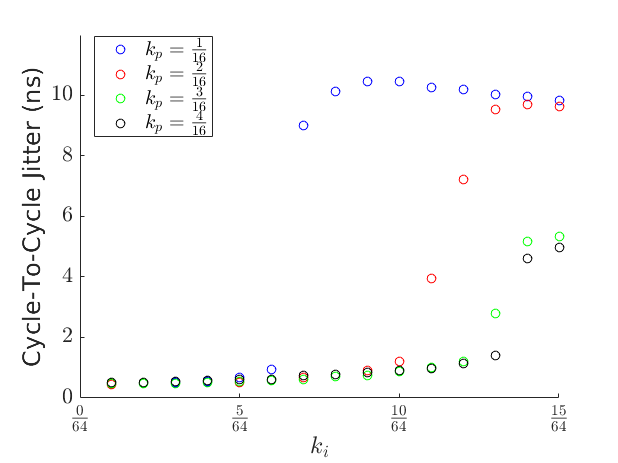
\includegraphics[width=0.6\textwidth]{../fixed_kp.png}
    \caption[Fixed $k_p$ integral gain sweeps]{Fixed $k_p$ integral gain sweeps.}
    \label{fig:gain_sweep}
\end{figure}
\begin{figure}[h]
    \centering
    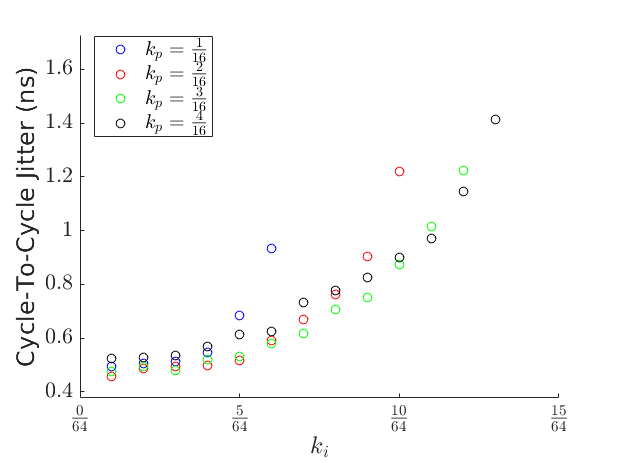
\includegraphics[width=0.6\textwidth]{../fixed_kp_zoom.png} 
    \caption[Fixed $k_p$ integral gain sweeps]{Fixed $k_p$ integral gain sweeps.}
    \label{fig:gain_sweep_zoom}
\end{figure}

Figure \ref{fig:gain_sweep} contains a sweep across the possible range of integral gains for four different proportional gains. This test was carried out with a 3x3 network of \ac{ADPLL} Design 3, each locked to the external reference at $5~\si{\mega\hertz}$. Only the generated waveforms from the \acp{ADPLL} at locations ``11'', ``22'' and  ``33'' were captured, alongside the external reference. It can be clearly observed that there are two distinct regions in the graph, with jitter values of less than $1~\si{\nano\second}$ contrasting sharply with the section where jitter is in the region of $10~\si{\nano\second}$. These distinct sections of the plot represent locked and unlocked operation respectively. Zooming in on the low jitter region in Figure \ref{fig:gain_sweep_zoom}, the approximate loss of lock thresholds can be compared with the theoretical relationship of $k_i = 0.5\times k_p$. The approximated loss of lock is determined as gain setting that caused the first \ac{ADPLL} to lose lock.
\begin{table}[!h]
    \begin{center}
        \begin{tabular}{lrr}
            \multicolumn{1}{c}{$k_p$} & \multicolumn{1}{c}{$k_i$} & \multicolumn{1}{c}{Ratio} \T\B\\
            \hline
            $\frac{1}{16}$            & $\frac{5}{64}$            & $0.8$ \T\B\\
            $\frac{2}{16}$            & $\frac{11}{64}$           & $0.72$ \T\B\\
            $\frac{3}{16}$            & $\frac{13}{64}$           & $0.92$ \T\B\\
            $\frac{4}{16}$            & $\frac{15}{64}$           & $1.07$ \T\B
        \end{tabular}
    \end{center}
    \vspace{-0.5cm}
    \caption[Loss of Lock Gains]{Loss of Lock Gains.}
    \label{table:lolgains}
\end{table}

Despite the relatively small number of proportional gains, it is clear that the exact relationship set out by Koskin does not hold in this system, but rather a scaled version of it does.  This difference is attributable to a modification in the structure of the \ac{LF}. In his simulations, the \ac{LF} design contains a register forming an input buffer, absent in the \ac{LF} used for these tests. The presence of this register, clocked on the generated signal, causes the \ac{ADPLL} to react more slowly to changes in the phase difference, thus increasing the jitter. This register was removed as it is not required to meet timing constraints in the \acp{ADPLL} used in this project. This removal allows the system to respond a cycle faster to a change in the phase relationships, and the impact of this change will be investigated further in a later section.

\subsection{Distribution of Period Steps}
To add context to the jitter numbers produced for each oscillator previously, the variation of period steps in the \ac{RO}, and delays in the \ac{TDL} due to implementation should be examined. The best way to visualise this distribution is through a histogram, placing periods within in a certain range into the same bin. This can be visualised effectively using Matlab's \texttt{histplot}. In order to obtain data, three instances of \acp{ADPLL} implementing each of the \ac{FPGA} clocked and inverter based \acp{DCO} were locked to an external reference signal at $5~\si{\mega\hertz}$. A capture was taken of each generated signal, the period of each clock cycle measured based on their rising edges.

\begin{figure}[h]%
    \centering
    \subfloat[Inverter propagation delay based \ac{RO}.]{{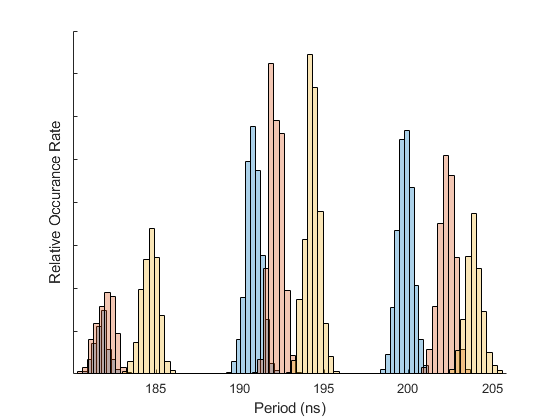
\includegraphics[width=0.5\textwidth]{../conf_paper/distrib_ring} }}%
    \subfloat[\ac{FPGA} clocked \ac{DCO}.]{{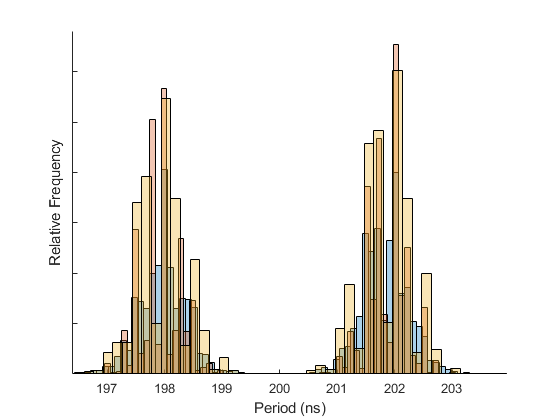
\includegraphics[width=0.5\textwidth]{../conf_paper/distrib_pa} }}%
    \caption[Example distribution of periods]{Example distribution of periods.}    
    \label{fig:dists}
\end{figure}
Figure \ref{fig:dists} contains the output of \texttt{histfit} for each of the three oscillators, superimposed in one plot for each \ac{DCO} type. As the \ac{RO} has significantly finer period resolution, the period steps would be overlaid on each-other, thereby making the plot difficult to read. In order to avoid this behaviour, the \ac{RO}'s mapping of control code to inverters was altered, from twice the control code to 16 times the control code. This resulted in a more pronounced separation of period steps while being indicative of the variation due to implementation.
The plots paint a a picture of the unrealistic nature of the \ac{FPGA} clocked design in comparison to its inverter based counterpart, as each \ac{DCO} has identical intrinsic period steps thus eliminating any jitter that may be seen in the system due to misalignment.
This effects the suitability of the FPGA clocked \ac{DCO} for the improvement of simulation models, or the examination of how a novel block may impact the behaviour of the network. If this analysis was carried out for the period steps, similar behaviour would be observed.


\subsection{\ac{FPGA} Clocked \ac{DCO} Width Variation}
When introducing the design of the \ac{DCO} for \ac{ADPLL} 1, the minimum possible accumulator width was chosen. From the equation used to calculate the frequency step size, it may have seemed that by doubling the bias point and increasing the width of the counter to 13 bits a finer resolution could be achieved.
\begin{align}
f_{step} &= \frac{f_{FPGA}}{2^{12}} = 62.988~\si{\kilo\hertz} \\
f_{step} &= \frac{f_{FPGA}}{2^{13}} = 31.494~\si{\kilo\hertz}
\end{align} Both the following measurements were carried out using identical loop filter gains, network configurations and reference signal. While in uni-directional mode some minor difference is observed in the maximum \ac{TIE}, but overall no statistically relevant changes were seen.

As Table \ref{table:accum_width} shows, while the resolution may have improved, the jitter has not. In this design, all signals are synchronised to the \ac{FPGA} clock, which has a $3.875~\si{\nano\second}$ period. The output waveform can only change at rising edges of the \ac{FPGA} clock, thus quantising the generated signal's period to increments of $3.875~\si{\nano\second}$. If the period step is shorter than the clock period, the extra resolution is lost and the \ac{FPGA} clock sets the minimum bound on the jitter. Accordingly, the most suitable counter width is that which maximises the number of bits, and thus achieves the best frequency resolution, with the constraint that, at the operating frequency, the period resolution is no finer than the \ac{FPGA} clock period. In this case, there is no bit width that satisfies both constraints, so the latter is relaxed to get a width of $12$.

\begin{table}[!ht]
    \begin{center}
        \begin{footnotesize}
            \setlength{\tabcolsep}{.9\tabcolsep}
            \begin{tabular}{ll|r|r|r|r|r|r|r|r|r|}           
                \cline{3-11}
                && \multicolumn{3}{c|}{Jitter Standard Deviation (ns)} & \multicolumn{3}{c|}{Max. Time Interval Error (ns)} & \multicolumn{3}{c|}{Skew (ns)} \T\\
                \cline{3-11} 
                &&PLL 11&PLL 12&PLL 22    &PLL 11&PLL 12&PLL 22    &PLL 11&PLL 12&PLL 22\T\\
                \hline
                \multicolumn{2}{|l|}{Accum. Width 12}&-&-&-&-&-&-&-&-&-\T\\
                \multicolumn{2}{|r|}{Uni-dir.}  &1.7693 &1.8463 &1.8862    &7.3060  &7.2565  &10.151    &2.2791 &1.2822  &1.6299  \T\\
                \multicolumn{2}{|r|}{Bi-dir.}   &1.9964 &1.9146 &1.9572    &15.0890 &18.2830 &19.673    &9.2449 &11.6120 &12.0520 \T\\
                \hline
                \multicolumn{2}{|l|}{Accum. Width 13}&-&-&-&-&-&-&-&-&-\T\\
                \multicolumn{2}{|r|}{Uni-dir.}  &1.7946 &1.8161 &1.9048    &6.8614  &7.1495 &9.371      &2.2257 &1.6328  &1.3778  \T\\
                \multicolumn{2}{|r|}{Bi-dir.}   &2.0016 &1.9217 &1.9605    &14.9580 &18.938 &19.510     &9.1678 &12.0000 &11.7690 \T\\
                \hline
                \B
            \end{tabular}
        \end{footnotesize}
        \caption{\acs{DCO} Accumulator Width Comparison.}
        \label{table:accum_width}
    \end{center}
    \vspace{-0.5cm}
\end{table}
%\FloatBarrier

\subsection{\ac{LF} Input Delay Register}\label{subsection:lf_delay}
Previously, when comparing the loss of lock gain relationship to that proposed by Koskin \textit{et al}, it was mentioned that the \ac{LF} used in this project does not have an input delay register. The lack of agreement between the theory and experimental results was attributed to the input delay register, or lack thereof. In order to provide a basis for this claim, the performance of a network in 2x2 configuration was analysed and the results of this analysis are presented in Table \ref{table:lf_delay}. While the \ac{C2C} jitter is statistically similar, there is significant difference to be observed in the \ac{TIE}, where an approximately $50\%$ increase can be observed, measurement for measurement. The absolute maximum \ac{TIE} is significantly impacted by the presence of any skew, as skew is the average value of this quantity, it is important to note that the skew has not meaningfully changed. As skew has not changed, it can be determined that jitter is the source of the increased \ac{TIE}.


It is in precisely this situation that \ac{C2C} jitter as a measurement is non-ideal. \ac{C2C} jitter does not differentiate between the situations in which the period variation is the same for multiple clock cycles in the same, or in opposite directions. \ac{C2C} jitter is therefore not a good indicator of how far apart the reference and generated signal's rising edges, whereas this is what \ac{TIE} is intended to do. As the delay due to the input register increases the reaction time of the \ac{ADPLL} to any changes in the reference, increases in the \ac{TIE} will be countered more slowly, thereby allowing the \ac{TIE} to grow for an extra clock cycle. Without a delay this is reacted to more quickly, limiting the maximum deviation. Both cases affect the same change in the period, just a cycle apart, so will impact the \ac{C2C} jitter identically.

\begin{table}[!ht]
    \begin{center}
        \begin{footnotesize}
            \setlength{\tabcolsep}{.9\tabcolsep}
            \begin{tabular}{ll|r|r|r|r|r|r|r|r|r|}           
                \cline{3-11}
                && \multicolumn{3}{c|}{Jitter Standard Deviation (ns)} & \multicolumn{3}{c|}{Max. Time Interval Error (ns)} & \multicolumn{3}{c|}{Skew (ns)} \T\\
                \cline{3-11} 
                &&PLL 11&PLL 12&PLL 22    &PLL 11&PLL 12&PLL 22    &PLL 11&PLL 12&PLL 22\T\\
                \hline
                \multicolumn{2}{|l|}{W/ \ac{LF} input reg}&-&-&-&-&-&-&-&-&-\T\\
                \multicolumn{2}{|r|}{Free PLLs} &0.66757 &0.84477 &0.71308    &5.9142 &6.1353 &5.3939   &-0.36997 &-0.20981 &-1.3344  \T\\
                \multicolumn{2}{|r|}{Uni-dir.}  &0.66934 &0.83894 &0.71271    &5.8779 &7.1746 &6.8914   &-0.36645 &-0.05647 &-0.36178 \T\\
                \multicolumn{2}{|r|}{Bi-dir.}   &0.68372 &0.83193 &0.68570    &7.5705 &9.6292 &9.7715   & 0.68901 & 1.58720 & 1.5553  \T\\
                \hline
                \multicolumn{2}{|l|}{W/o \ac{LF} input reg}&-&-&-&-&-&-&-&-&-\T\\
                \multicolumn{2}{|r|}{Free PLLs} &0.67899 &0.65618 &0.61415    &4.2527 &3.6478 &3.8483   &-0.31418 &0.11897 &-0.57619 \T\\
                \multicolumn{2}{|r|}{Uni-dir.}  &0.68534 &0.69405 &0.63666    &4.3257 &4.2901 &4.6185   &-0.38849 &0.23363 & 0.21156 \T\\
                \multicolumn{2}{|r|}{Bi-dir.}   &0.68248 &0.70175 &0.61356    &5.3497 &6.2640 &6.8079   & 0.52553 &1.7025  & 1.9499  \T\\
                \hline
                \B
            \end{tabular}
        \end{footnotesize}
        \caption{Impact of \ac{LF} Input Delay Register.}
        \label{table:lf_delay}
    \end{center}
    \vspace{-0.5cm}
\end{table}
%\FloatBarrier

\subsection{Impact of Frequency Divider}
The major benefit of \iac{PLL} network over other forms of coupled oscillator based clock distribution systems is that the coupling can be done using a signal significantly reduced in frequency, thereby reducing the power consumption of the related hardware. It is important, therefore, to ensure that the insertion of a feedback divider does not introduce any further jitter to the system. Table \ref{table:div} presents the results of measurements at a number of division levels. As re-implemenation was performed between each measurement, there is some variation present. However, it is notable that for each \ac{ADPLL} that saw \iac{C2C} jitter increase, there was another that performed better than at a lower level of division. Accordingly, it can be claimed that the insertion of a feedback divider does not impact the \ac{C2C} jitter present. Intuitively this makes sense as the control code will change more violently, but proportionally less frequently. 
\begin{table}[!ht]
    \begin{center}
        \begin{footnotesize}
            \setlength{\tabcolsep}{.9\tabcolsep}
            \begin{tabular}{ll|r|r|r|r|r|r|r|r|r|}           
                \cline{3-11}
                && \multicolumn{3}{c|}{Jitter Standard Deviation (ns)} & \multicolumn{3}{c|}{Max. Time Interval Error (ns)} & \multicolumn{3}{c|}{Skew (ns)} \T\\
                \cline{3-11} 
                &&PLL 11&PLL 12&PLL 22    &PLL 11&PLL 12&PLL 22    &PLL 11&PLL 12&PLL 22\T\\
                \hline
                \multicolumn{2}{|l|}{No Divider}&-&-&-&-&-&-&-&-&-\T\\
                \multicolumn{2}{|r|}{Free PLLs} &0.66757 &0.84477 &0.71308    &5.9142 &6.1353 &5.3939    &-0.36997 &-0.20981 &-1.3344  \T\\
                \multicolumn{2}{|r|}{Uni-dir.}  &0.66934 &0.83894 &0.71271    &5.8779 &7.1746 &6.8914    &-0.36645 &-0.05647 &-0.36178 \T\\
                \multicolumn{2}{|r|}{Bi-dir.}   &0.68372 &0.83193 &0.68570    &7.5705 &9.6292 &9.7715    & 0.68901 & 1.58720 & 1.5553  \T\\
                \hline
                \multicolumn{2}{|l|}{Divide by 2}&-&-&-&-&-&-&-&-&-\T\\
                \multicolumn{2}{|r|}{Free PLLs} &0.68252 &0.51750 &1.1074     &4.9464 &4.0728 &6.7426    &-0.91985 &-1.7024  &-1.84279 \T\\
                \multicolumn{2}{|r|}{Uni-dir.}  &0.68441 &0.53203 &1.1081     &4.8707 &4.9684 &8.9973    &-0.99034 &-1.0240  &-0.63989 \T\\
                \multicolumn{2}{|r|}{Bi-dir.}   &0.69524 &0.54953 &1.1033     &6.8180 &7.8760 &12.288    & 0.00337 & 0.69148 & 1.3085  \T\\
                \hline
                \multicolumn{2}{|l|}{Divide by 4}&-&-&-&-&-&-&-&-&-\T\\
                \multicolumn{2}{|r|}{Free PLLs} &0.77564 &0.55934 &0.65770    &10.576 &6.7330 &12.647    &-1.1507  &-1.8670   &-2.3381 \T\\
                \multicolumn{2}{|r|}{Uni-dir.}  &0.77443 &0.56544 &0.66019    &10.210 &7.4612 &15.166    &-1.2283  &-1.2691   &-1.0948 \T\\
                \multicolumn{2}{|r|}{Bi-dir.}   &0.77657 &0.57043 &0.66809    &11.408 &10.859 &17.242    &-0.28439 & 0.40697  & 0.8351 \T\\
                \hline
                \B
            \end{tabular}
        \end{footnotesize}
        \caption{Network Performance at Different Divider Levels.}
        \label{table:div}
    \end{center}
    \vspace{-0.5cm}
\end{table}
%\FloatBarrier

It does have a significant impact on the maximum \ac{TIE}, however, and notably this occurs without any meaningful change in skew. This confirms an increase in jitter due to the greater division levels as the source of the performance degradation. This can be explained by examining how the dividers behave. When a divider is inserted into the network, the phase error is computed at a greatly reduced rate. This means the rate at which the \ac{LF} is updated also drops, and therefore the control code changes $n$ times less frequently, where $n$ is the division level. The dividers reduce the speed at which the individual \acp{ADPLL} can react to a phase difference, while locking the resulting control code in place for a ever greater number of clock cycles as the division level increases. This greater duration may cause a control code to be applied for an excessively long number of cycles, resulting in a drift of the rising edge of the divided/generated signal away from the reference, which will manifest as \ac{TIE}. These tests were carried out with identical gains for the proportional and integral paths in order to demonstrate the effect, however, an appropriate reduction in these gains can correct this problem by reducing the magnitude of the control code alteration.
%TODO ask mulkeen
Figure \ref{fig:todo_div} can confirm this behaviour. In Plot (a), as the division level increases, the number of cycles spent at a $200~\si{\nano\second}$ period decreases. This confirms that overcorrection is occurring, thus resulting in the increased \ac{TIE} seen in Plot (b).
\begin{figure}[h]%
    \centering
    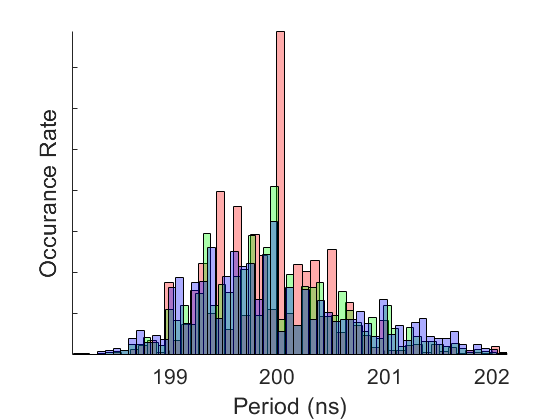
\includegraphics[width=0.8\textwidth]{../dist2}
    \caption[Period distribution at different divider levels]{Period distribution at different divider levels.}    
    \label{fig:todo_div}
\end{figure}

\section*{\acs{ADPLL} Use Cases}
As each design was introduced, the most appropriate use cases for that particular \ac{ADPLL} were suggested. \ac{ADPLL} networks can be used in a number of roles: from modelling system dynamics or the refinement of behavioural simulation models to the validation, verification and testing of potential \ac{ASIC} based networks (Zianbetov \& Shan) or the design of other hardware for the purposes of network performance improvement or control. However, some architectures of \ac{ADPLL} are more suited to particular roles than others.

As mentioned when \ac{FPGA} clocked designs were introduced, their configurability made them particularly suited to the validation and verification of designs destined for use in \acp{ASIC}, as was the case with Zianbetov and Shan \cite{zianbetov2013phd,shan2014phd}. In contrast to the \ac{RO} based designs, in which configurability is more more restricted, it is possible to replicate the resolution, centre frequencies and other \ac{ADPLL} characteristics of the design requiring verification at a scaled down frequency. This can be carried out at large division ratios, where the \ac{FPGA} clock period is not a restricting factor, such as the $50~\si{\kilo\hertz}$ centre frequency used by Zianbetov and Shan. In order to reduce the frequency to this extent with inverters, over $30,000$ would be required, introducing the potential for even greater variation in \ac{DCO} centre frequencies due to implementation. The other issue arising from this number of inverters, is the floorspace of the \ac{FPGA} that would be consumed implementing just one \ac{RO}. In the case of the Xilinx \acl{Nexys}, and extrapolating based on the resource usage of the $373$ inverter \acp{RO} implemented, a single \ac{RO} would consume half the look-up tables available, eliminating the possibility of a network.

While the \ac{FPGA} based designs feature characteristics which make them particularly suitable for use as a validation tool, their performance in a network reduces their suitability for the refinement of software based simulations, or in the analysis of new control or performance enhancement tools. Referring back to Table \ref{table:2x2perf}, not only is \ac{C2C} jitter significantly greater than the inverter based designs, a large degree of skew is also present. These combined make \ac{FPGA} clocked designs unsuitable for the aforementioned purposes. In particular, as seen with the increase to a 3x3 network, this skew becomes the limiting factor the network size.

Figure \ref{fig:dists}, which demonstrated the impact of period distribution, highlights a second major unrealistic behaviour present in \ac{FPGA} clocked \ac{ADPLL} designs, as \iac{ASIC} destined design will not exhibit this identical linear period distribution. While \ac{ADPLL} 2 will feature a large degree of variation due to implementation differences, these differences are only present in the \ac{RO} not the \ac{PFD}. As testing Designs 2 \& 3 has shown, particularly the results displayed in Table \ref{table:2x2perf}, apart from a larger skew, the jitter performance is quite similar, meaning that the extra complexity of inverter based \ac{PFD} is not required, for smaller networks, in order to achieve as accurate behaviour as can be achieved in this environment. The implementation based variation of the detector step manifests itself as an increase in the jitter across all network modes, as would be expected, compared to the \ac{FPGA} based design.

Accordingly, if the aim of this platform is the enhancement of a model, the validation of theoretical results or the analysis of the performance of new control or performance enhancement hardware, the \ac{RO} based designs are idea for this purpose. Two members of the research team here in \acs{UCD}, Eugene Koskin and Pierre Bisiaux, have been using \iac{ADPLL} with the same architecture as Design 3, for these very purposes.



\setcounter{chapter}{5}

\chapter{Conclusion}\label{chap:6}

\section{Conclusions}
\section{Impact of Research}
\section{Suggested Future Work}

\setcounter{chapter}{6}

\pagebreak{}
\phantomsection
\addcontentsline{toc}{chapter}{Bibliography}
\fancyhead[LO,RE]{\slshape \nouppercase{\leftmark}}\bibliographystyle{IEEEtran}
\bibliography{thesis}

\end{document}
